\section{Hierarchical Generative Graph Diffusion}
\label{sec: higendiff}

In the previous section, we discussed how GGG-CRP, an autoregressive permutation-equivariant GAN, was able to come close to the performance of the baseline network with much less memory complexity. However, the approach still suffered from lower generalization to certain graph structures, an issue common with autoregressive models for graphs \cite{krawczuk_gg-gan_2020}. We predict this is due to the overly holistic idea of sampling the community structures via simple categorical distributions and integer partition probabilities, as well as the general difficulty of GAN fine-tuning. 

The correct approach, no matter the task, as hinted in the introduction, is always to assign complete machine learning models for both coarse and fine levels of graph data, i.e., learn the distribution of community graphs, inter-community graphs, and further coarsenings in order to sample all these graph views accurately, and it was not believed that a collection of conditional GANs could tackle this challenge. In fact, shortly after the work on GGG-CRP, a different class of generative models arose as state-of-the-art for graph generation performance: \emph{diffusion models}. The text in this section thus introduces HiGenDiff (Hierarchical Generative Diffusion) models for both highly scalable and powerful graph distribution representation, even when graph samples reach non-elementary sizes. Specifically, we will extend the work of \cite{vignac_digress_2022}, \cite{karami_higen_2024}, \cite{karami_multi-resolution_2024}, and \cite{krawczuk_graph_2024} with new model designs, theoretical analyses, and improved experimental results.

\subsection{Motivation}
Despite remarkable achievements on small and medium-sized graphs (e.g., molecules, proteins) encounter scalability challenges when applied to larger, more complex structures like social networks, financial networks, road networks, and electronic circuits \cite{krawczuk_graph_2024}. 

Real-world networks often exhibit locally heterogeneous patterns, where communities of nodes tightly connect within themselves, but there exist sparse inter-connections between groups.
This naturally forms a hierarchical multi-resolution structure in graphs, with smaller communities nested within larger ones. In such a structure, lower levels capture fine-grained local interactions within communities, while higher levels represent broader relationships between communities and
the overall network structure. Therefore, to truly capture the complexity of such graphs, it is crucial for an expressive graph generative network to not only learn these community structures but also to model how they interact across different levels. By incorporating this inductive bias into the model architecture, we can train an expressive generative model that can effectively capture the hierarchical structure inherent in graphs \cite{karami_multi-resolution_2024}. 

This work thus introduces HiGenDiff (Hierarchical Generative Diffusion), which exploits the community structure and multi-resolution hierarchy inherent in many real-world graph datasets to tackle this complexity while preserving expressiveness.

\subsection{Background}

\begin{definition}
    Given a set of samples $\mathcal{D}=\offf{\mathbf{X}_i}_{i=1}^{N}$ and $T\in\mathbb{N}$, a \emph{diffusion model} \cite{sohl-dickstein_deep_2015} $\mathcal{M}=\offf{\offf{f_t}_{t=1}^{T},\offf{g_t}_{t=1}^{T}}$ assumes that there exists a finite $T$-step Markov stochastic process $\offf{\mathbf{X}_t}_{t=0}^{T}$, where $\mathbf{X}_0 \in \mathcal{D}$ and $\mathbf{X}_T \sim Z$ (i.i.d. random noise). 

    In the most common design, the stochastic process is defined as $\mathbf{X}_t=\alpha_t \mathbf{X}_{0} + \beta_t \varepsilon_t $, with $\varepsilon_t \sim Z$, $\offf{\alpha_t}_{t=0}^{T}$ non-increasing, $\offf{\beta_t}_{t=0}^{T}$ non-decreasing.
    
    Each $f_t: \mathbb{R}^F \times \mathbb{R}^F \to \mathbb{R}$ models the conditional probability $\mathbb{P}\of{\mathbf{X}_{t-1}\mid \mathbf{X}_t}$, so as to model the sample likelihood via the Markov property:
    \begin{equation}
    \mathbb{P}\of{\mathbf{X}_0 \in \mathcal{D}}=\mathbb{P}\of{\mathbf{X}_T}\prod_{t=1}^{T}{\mathbb{P}\of{\mathbf{X}_{t-1} \mid \mathbf{X}_t}}=\mathbb{P}\of{Z}\prod_{t=1}^{T}{\sigma\of{f_t\of{\mathbf{X}_{t-1}, \mathbf{X}_t}}}
    \end{equation}
    
    On the other hand, each generator model $g_t:\mathbb{R}^F \to \mathbb{R}^F$ is trained to reverse one step of the stochastic process in order to obtain a dataset sample from random noise (i.e., all are denoising models that output $\forall t, \hat{\mathbf{X}}_{t-1}=g_t\of{\hat{\mathbf{X}}_t}$):
    \begin{align}   
    \begin{split}
    \forall t, g_t &= \argmin_{g}{\mathbb{E}_{\mathcal{D},Z}\off{-\log{\mathbb{P}\of{g\of{\mathbf{X}_t}\mid\mathbf{X}_t}}}}=\argmin_{g}{\mathbb{E}_{\mathcal{D},Z}\off{-\log{\sigma\of{f_t\of{g\of{\mathbf{X}_t},\mathbf{X}_t}}}}} \\
    \hat{\mathbf{X}}_0 &= \of{g_T \circ g_{T-1}\circ\dots\circ g_1}\of{\hat{\mathbf{X}}_T},\hat{\mathbf{X}}_T\sim Z
    \end{split}
    \end{align}
\end{definition}

As an extension of DiGress \cite{vignac_digress_2022}, HiGenDiff sub-models also employ the non-standard \emph{discrete stochastic process}. Namely, it is standard to employ standard Gaussian noise $Z\sim N\of{\mathbf{0},\mathbf{I}_F}$ for the latent noise distribution of diffusion models and one-dimensional reals for $\alpha_t,\beta_t$. However, all models based on DiGress acknowledge the discrete nature of graph distributions and use the following formula for the Markov chain of e.g., a given node feature value:
\begin{align}
\begin{split}
    \of{\mathbf{X}_i}_t &\sim \text{Categorical}\of{Q_t \cdot \text{OneHot}\of{\of{\mathbf{X}_i}_0}} \\
    Q_t &= \alpha_t \mathbf{I}_F + \beta_t \hat{Q},
\end{split}
\end{align}
where $\hat{Q} \in \off{0,1}^{F \times F}$ is a transition matrix representing staying in the state of the \emph{estimated marginal distribution} of the features in $\mathcal{D}$, i.e. $\forall i,j,\hat{Q}_{i,j} = \hat{p}_j$, $\sum_{j=1}^{F}{\hat{p}_j}=1$. For the edge features, analogously replace $F$ with $\abs{R}+1$. In this manner, the diffusion model learns to smoothly interpolate between graphs with random node and edge features sampled according to marginal probabilities and graphs with structure, through the probabilistic flipping of random nodes or edges.

Given a dense representation of a graph sample $\of{\mathbf{X},A}$, where $n$ is the number of nodes, $\mathbf{X} \in \mathbb{R}^{n \times F}$ are the node features and $A \in \offf{0,1,\dots,\abs{R}}^{n \times n}$ is the edge-label-enriched adjacency matrix, HiGenDiff represents the graph's \emph{hierarchical community structure} $\off{G^{\of{l}}}_{l=1}^{L}=\off{\of{\mathbf{X}^{\of{l}},A^{\of{l}}}}_{l=1}^{L}$ as the collection $G=\of{G_R,\off{\of{M^{\of{l}}, \offf{C^{\of{l}}_{k}}_{k=1}^{n^{\of{l+1}}},\offf{B^{\of{l}}_{j,k}}_{j \neq k}}}_{l=1}^{L-1}}$, where:
\begin{itemize}
    \item $L \in \mathbb{N}$ is the number of levels in the hierarchy;
    \item $n^{\of{l}}$ is the number of nodes in the $l$-th level of the hierarchy, $n^{\of{1}}=n$;
    \item $M^{\of{l}} \in \offf{0,1}^{n^{\of{l+1}} \times n^{\of{l}}}$ is the community assignment matrix, dictating how to coarsen the $l$-th level nodes into the $l+1$-th level nodes:
    \begin{align}
        \begin{split}
            \mathbf{X}^{\of{l+1}}&=M^{\of{l}} \cdot \mathbf{X}^{\of{l}} \\
            A^{\of{l+1}}&=\begin{cases}
                M^{\of{l}} \cdot A^{\of{l}} \cdot {M^{\of{l}}}^T, & l>1 \\
                M^{\of{l}} \cdot \bar{A}^{\of{l}} \cdot {M^{\of{l}}}^T, & l=1
            \end{cases},
        \end{split}
    \end{align}
    where $\forall i,j, \bar{A}^{\of{l}}_{i,j}=\mathbb{I}\of{A^{\of{l}}_{i,j}>0}$
    \item $G^{\of{1}}=\of{\mathbf{X}^{\of{1}},A^{\of{1}}}=\of{\mathbf{X},A}$, the original input graph is on the lowest level;
    \item $G_R=G^{\of{L}}=\of{\mathbf{X}^{\of{L}}, A^{\of{L}}}$ is the \emph{root graph}, the top level of the hierarchy that does not have further coarsenings;
    \item $\offf{C^{\of{l}}_{k}}_{k=1}^{n^{\of{l+1}}}$ is the set of \emph{community subgraphs} of the graph at level $l$;
    \item $C^{\of{l}}_{k}=\of{\mathbf{X}_k^{\of{l}},A_k^{\of{l}}}$, where $\mathbf{X}_k^{\of{l}}=\off{\mathbf{X}_i^{\of{l}}}_{M^{\of{l}}_{k,i}=1}$ and $A_k^{\of{l}}=\off{A_{i,j}^{\of{l}}}_{M^{\of{l}}_{k,i}=M^{\of{l}}_{k,j}=1}$
    \item $\offf{B^{\of{l}}_{j,k}}_{j \neq k}$ is the set of \emph{bipartite inter-community subgraphs} of the graph at level $l$;
    \item $B^{\of{l}}_{j,k}=\of{\mathbf{X}_{j,k}^{\of{l}},A_{j,k}^{\of{l}}}$, where $\mathbf{X}_{j,k}^{\of{l}}=\off{\mathbf{X}_{j}^{\of{l}},\mathbf{X}_{k}^{\of{l}}}$ and $A_{j,k}^{\of{l}}=\off{A_{h,i}^{\of{l}}}_{M^{\of{l}}_{j,h}=M^{\of{l}}_{k,i}=1}$.
\end{itemize}

Figure \ref{fig:higendiff} provides a visual representation of an example hierarchical structure, to aid the understanding of the above description.
\begin{figure}[H]
    \centering
    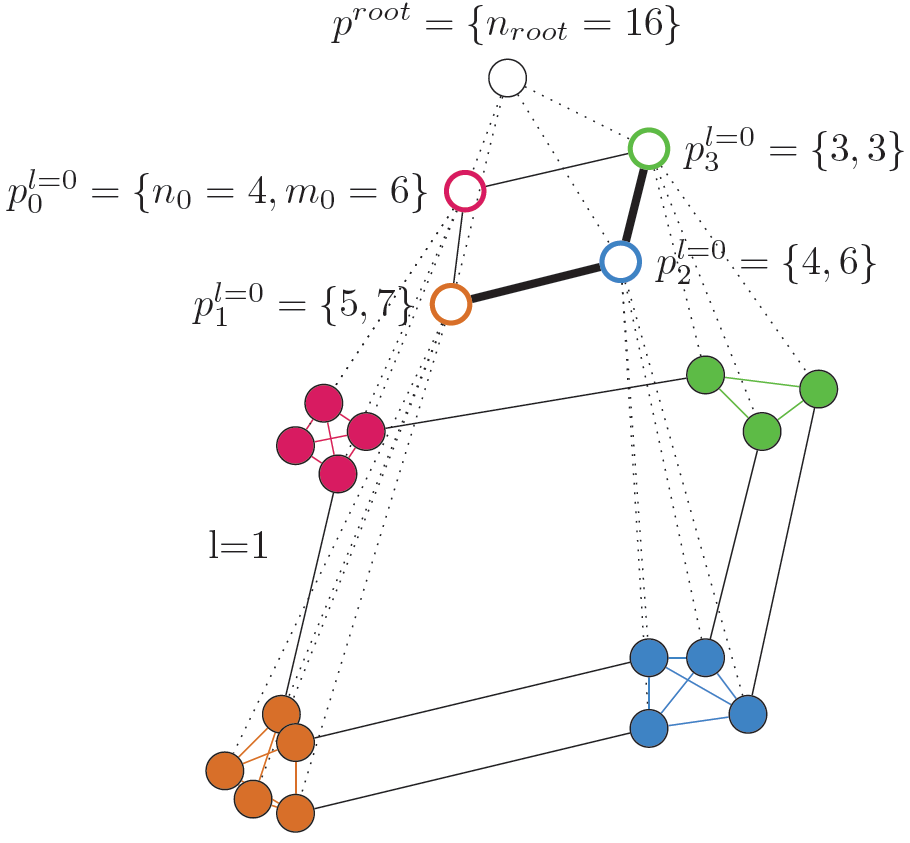
\includegraphics[width=0.35\linewidth]{figures/higendiff/hierarchical_graph.png}
    %\hfill
    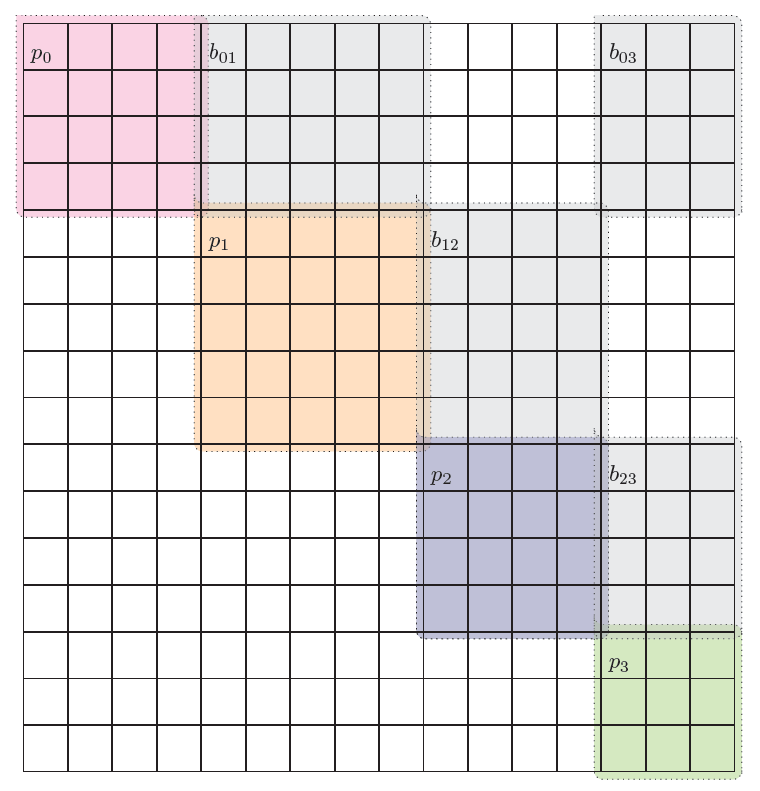
\includegraphics[width=0.35\linewidth]{figures/higendiff/hierarchical_adj.png}
    \caption[Node-edge drawing and adjacency block visualization of a hierarchical graph structure.]{Node-edge drawing and adjacency block visualization of a hierarchical graph structure, with labeled aggregate node and edge counts, the additional features that HiGenDiff employs. Color-shaded areas denote the community subgraphs, gray shaded areas are the bipartites (mirrored on the lower triangular), and unshaded areas are skipped during diffusion of the current level, according to the result of the previous level. Credit to \cite{karami_multi-resolution_2024}.}
    \label{fig:higendiff}
\end{figure}
Given a dataset $\mathcal{D}=\offf{G_i}_{i=1}^{N}$ of such hierarchical graph structures, HiGenDiff employs MRGrad's model architecture \cite{karami_multi-resolution_2024} to learn that distribution. Namely, HiGenDiff is comprised of $2L-1$ diffusion models: $\mathcal{M}=\of{\mathcal{M}_P,\off{\of{\mathcal{M}^{\of{l}}_C,\mathcal{M}^{\of{l}}_B}}_{l=1}^{L-1}}$, where $\mathcal{M}_P$ learns to sample from the distribution of root graphs, while $\mathcal{M}^{\of{l}}_C$ and $\mathcal{M}^{\of{l}}_B$ learn the $l$-th level's community and bipartite distributions, respectively, $\forall l<L$. 

For the likelihood modeling, we employ the independence property between community and bipartite graphs when conditioning on a given upper-level coarsening, yielding:
\begin{equation}
\mathbb{P}\of{G \in \mathcal{D}}=\mathbb{P}\of{G^{\of{L}}}\prod_{l=1}^{L-1}{\mathbb{P}\of{G^{\of{l}} \mid G^{\of{l+1}}}}=\mathbb{P}\of{G_R}\prod_{l=1}^{L-1}\prod_{k=1}^{n^{\of{l+1}}}{\mathbb{P}\of{C_{k}^{\of{l}} \mid G^{\of{l+1}}}}\prod_{l=1}^{L-1}\prod_{j \neq k}{\mathbb{P}\of{B_{j,k}^{\of{l}} \mid G^{\of{l+1}}}}     
\end{equation}

For the sampling models, similar to MRGrad:
\begin{itemize}
    \item $\mathcal{M}_P$ is a DiGress diffusion model \cite{vignac_digress_2022}, modified to support generation of general weighted graphs. Root graphs are sampled with such an architecture independently, as the first step of HiGenDiff. We will present the different methods for modeling and diffusing edge weights in the next subsection, as this was found to be a very important ablation dimension. 
    \item Each $\mathcal{M}^{\of{l}}_C$ community generator is a graph transformer model with the architecture of \cite{dwivedi_generalization_2021}, modified to support conditioning on the features of a parent graph. For each level, community graphs are sampled independently before the bipartites.
    \item Each $\mathcal{M}^{\of{l}}_B$ bipartite generator is a GraphGPS model \cite{rampasek_recipe_2022}, customized to have a linear complexity of adjacency matrix generation w.r.t. the number of input nodes and to support conditioning on the features of a parent graph. Bipartites are generated jointly after the communities for each level, in order to align the inter-community edges more accurately.
\end{itemize}

\subsection{Contributions}

\subsubsection{Model}
We extend MRGrad's model design with a more detailed exploration of the same variables in the diffusion model architecture. Namely, we also agree on the significance of the first, root graph, diffusion step on the overall quality of the final sampled hierarchical graph structures. As such, we describe the $\mathcal{M}_R$ model variations below, where the differences lie in how accurately the edge weights of the root graph, $A^{\of{L}}$, are modeled:
\begin{itemize}
    \item \textbf{Simple}: In this setting, we completely replace $A^{\of{L}}$ with $\bar{A}^{\of{L}} \in \offf{0,1}^{n^{\of{L}} \times n^{\of{L}}}$, the simple binary discretization of the root weights described previously. This thus has implications for the discrete stochastic process, where now $\hat{Q}\in\off{0,1}^{2 \times 2}$ for each adjacency entry of the root. This configuration is the one with the least representation power;
    \item \textbf{Integer}: In this setting, we acknowledge that the root graph's weights can be any non-negative integers from 0 to the number of edges in the graph $\abs{E}$. This is essentially the default setting, where we fully generate the original $A^{\of{L}} \in \offf{0,1,\dots,\abs{E}}^{n^{\of{L}} \times n^{\of{L}}}$, and $\hat{Q}\in\off{0,1}^{\of{\abs{E}+1} \times \of{\abs{E}+1}}$;
    \item \textbf{Ordinal}: The most accurate noising process of the root weights is the one that would acknowledge their \emph{ordered} nature, i.e., it should be very unlikely for a very high edge weight to be instantly flipped to 0 in one step. The ordinal setting acknowledges this and modifies $\hat{Q} \in \off{0,1}^{\of{\abs{E}+1} \times \of{\abs{E}+1}}$ to be \enquote{Markov-like} and allow only transitions to neighboring integers on the number line: 
    \begin{equation}
        \hat{Q}_{i,j}=\begin{cases}
            \hat{p}_j, & \abs{i-j}\leq 1 \\
            0, & \text{otherwise}
        \end{cases}
    \end{equation}
    \item \textbf{Bucketization}: When $\abs{E}$ is large, the Integer and Ordinal variants could struggle with high computational cost and/or overfitting of the root graph distribution, due to the large amount of required parameters to model the root weight values in high detail. We thus propose an option to discretize the set $\offf{0,1,\dots,\abs{E}}$ into $W<\abs{E}$ buckets, and allow transitions only between buckets. Formally, given the bucket boundaries $\offf{b_i}_{i=0}^{W+1}$ where $b_0=0,b_1=1,b_{W+1}=\abs{E}$, we compute the discretized adjacencies $\tilde{A}^{\of{L}} \in \offf{0,1,\dots,W}^{n^{\of{L}} \times n^{\of{L}}}$ as $\tilde{A}_{i,j}^{\of{L}}=w \Leftrightarrow b_w < A_{i,j}^{\of{L}} \leq  b_{w+1}$. With bucketization active, $\hat{Q} \in \off{0,1}^{\of{W+1} \times \of{W+1}}$.
\end{itemize}

\subsubsection{Theory}
From how we described the likelihood modeling of HiGenDiff in the previous subsection, the similarities with the COINs technique for scalable knowledge graph query-answer ranking are evident. What a bi-level HiGenDiff model performs to score and generate root graph, community, and bipartite adjacencies is analogous to the application of COINs' community, intra-community, and inter-community models for query-answer pair likelihood, respectively. Keeping this in mind, one can ask the same theoretical questions we posed for COINs: 
\begin{center}
    \emph{What is the computational cost of adding an extra graph coarsening layer on top, and when is this feasibly faster than the standard baseline?}
\end{center}
Proposition \ref{proposition:complexity_higendiff} provides an answer to the first question, under certain assumptions. The proof is available in Appendix \ref{sec:appendix_higendiff_theory}. Note that the quadratic cost of generating the dense adjacency matrices dominates the cost of sampling node features, which is linear (w.r.t. number of nodes). Thus, when discussing the computational complexity of dense graph generation, we only focus on how the cost for edges is affected.

\begin{proposition}
    \label{proposition:complexity_higendiff}
    Let $L \geq 1$ be the current top level of the graph hierarchy, and $M^{\of{L}} \in \offf{0,1}^{n^{\of{L+1}}\times n^{\of{L}}}$ the node-community assignment matrix for the proposed coarsening of the current $n^{\of{L}}$-node graph into $n^{\of{L+1}}$ communities. Under the assumption that, after obtaining $A^{\of{L+1}}=M^{\of{L}} \cdot A^{\of{L}} \cdot {M^{\of{L}}}^T$, $\bar{A}_{i,j}^{\of{L+1}} \overset{\text{i.i.d.}}{\sim} \text{Bernoulli}\of{p}$, then the expected computational cost of generating the $L$-th level while being aware of the hierarchy has the following form and bounds:
    \begin{equation}
         \frac{3}{2}\mathbb{E}\off{\sqrt[3]{2{n^{\of{L}}}^4}} \leq \mathbb{E}\off{{n^{\of{L+1}}}^2} + p \mathbb{E}\off{{n^{\of{L}}}^2} \leq 2\mathbb{E}\off{{n^{\of{L}}}^2}
    \end{equation}
\end{proposition}

So $\mathcal{O}({n^{\of{L}}}^{\frac{4}{3}})$ is the best sub-quadratic cost we can achieve by adding the $L+1$-st level, which is non-trivial, as it implies there is a large enough window of possible acceleration values communities of sufficient quality can achieve. However, if the current root graph has a highly dense inter-community interaction graph, then unfortunately HiGenDiff will have a \emph{twice} greater cost to generate it. The threshold for feasibility is quantified by Proposition \ref{proposition:feasibility_higendiff} below.

\begin{proposition}
\label{proposition:feasibility_higendiff}
     Let $L \geq 1$ be the current top level of the graph hierarchy. Under the assumption of Proposition \ref{proposition:complexity_higendiff}, coarsening the graph once again and adding an $L+1$-st level is feasible if and only if:
     \begin{equation}
            p < 1 - \frac{\mathbb{E}\off{{n^{\of{L+1}}}^2}}{\mathbb{E}\off{{n^{\of{L}}}^2}}
     \end{equation}
\end{proposition}
\begin{proof}
    By Proposition \ref{proposition:complexity_higendiff}, $\mathbb{E}\off{{n^{\of{L+1}}}^2} + p \mathbb{E}\off{{n^{\of{L}}}^2}$ is the expected cost for HiGenDiff, while we know the baseline cost is just $\mathbb{E}\off{{n^{\of{L}}}^2}$. So we are faster in expectation when:
    \begin{align}
        \begin{split}
            \mathbb{E}\off{{n^{\of{L+1}}}^2} + p \mathbb{E}\off{{n^{\of{L}}}^2} &< \mathbb{E}\off{{n^{\of{L}}}^2} \\
            p \mathbb{E}\off{{n^{\of{L}}}^2} &< \mathbb{E}\off{{n^{\of{L}}}^2} - \mathbb{E}\off{{n^{\of{L+1}}}^2}  \\
            p &< 1 - \frac{\mathbb{E}\off{{n^{\of{L+1}}}^2}}{\mathbb{E}\off{{n^{\of{L}}}^2}}
        \end{split}
    \end{align}
\end{proof}

\subsubsection{Experiments}

Our experiment setup for HiGenDiff follows closely that of \cite{karami_multi-resolution_2024}. This includes computing hierarchical structures of graphs using the Louvain community detection algorithm \cite{blondel_fast_2008}, and measuring generation performance by comparing sampled and true distributions of degrees, clustering coefficients, eigenvalues, and orbit sizes. We employ the standard Maximum Mean Discrepancy (MMD) test \cite{gretton_kernel_2012} for evaluating distribution distance. 

As notable differences, we single out our more extensive model ablation and the addition of two new datasets of graphs with interesting community structure.

Namely, we have the choice of building 5 different diffusion configurations: Simple, Integer, Integer-Bucketized, Ordinal, and Ordinal-Bucketized. We also investigated the need whether bipartite graphs really need to be diffused jointly, as well as the need for conditional probability modeling between hierarchy levels, thus the need for three different modified graph transformers. As an alternative, we constructed the Naive setup, where all HiGenDiff sub-models are independent DiGress instances, generating graph parts independently, which are then stitched into a final graph with simple concatenation.

Each of the model configurations, except the Naive, was trained and evaluated on the 4 datasets chosen by MRGrad: a dataset of Stochastic Block Model (SBM) samples provided by \cite{martinkus_spectre_2022}, the CiteSeer ego networks of \cite{sen_collective_2008}, and the 2 protein structure datasets enzyme \cite{schomburg_brenda_2004} and DD2 \cite{dobson_distinguishing_2003}, classical for drug discovery. We also present HiGenDiff performance results on datasets of:
\begin{itemize}
    \item 1000 sampled ring-of-cliques graphs, with the number of cliques ranging from 3 and 10 and the clique size ranging from 3 to 5, referred to as RoC;
    \item 1000 sampled graphs according to the LFR benchmark \cite{lancichinetti_finding_2011}, with parameters $\tau_1=3, \tau_2=1.5, n \sim \text{Uniform}\of{\off{100, 250}}, \mu \sim \text{Uniform}\of{\off{0.03, 0.75}}$.
\end{itemize}

\subsection{Results}

We begin by presenting the results of the Louvain community detection for each of the 6 datasets in Table \ref{tab:higendiff_datasets}. The main important finding is that only 2 levels were sufficient for each dataset, and this is due to the relative scale of the graph sizes involved. 

Nevertheless, with graph sizes in the hundreds, as the ones we considered, non-hierarchy-aware models like DiGress will already fail to scale in performance and speed. We can observe that for all but one of the datasets, HiGenDiff provided meaningful speed-up factors on average. The outliers are the SBM graphs, which had almost surely cliques as their root graphs, and thus, the set of bipartite graphs to be generated grew quadratically.

For the same reason, SBM graphs are highly likely to be infeasible. We stress, however, that only for the SBM graphs and rings of cliques can one prove that the Bernoulli assumption of Propositions \ref{proposition:complexity_higendiff} and \ref{proposition:feasibility_higendiff} is satisfied. Regardless, the theoretical result provides us with a rough estimate of the true feasibility, which is highly invaluable: the important protein structure datasets are shown to be almost surely very appropriate candidates for HiGenDiff speed-ups.

\begin{table}[H]
    \centering
    \caption[Statistics from the hierarchical structure of the HiGenDiff datasets.]{Statistics from the hierarchical structure of the HiGenDiff datasets. Left to right: number of nodes, number of communities, root graph density, speed-up factor compared to the baseline cost, and the probability of a graph satisfying Proposition \ref{proposition:feasibility_higendiff}.}
    \label{tab:higendiff_datasets}
\begin{tabular}{lrrrrr}
\toprule
Dataset & $n^{\of{1}}$ & $n^{\of{2}}$ & $p$ & Acceleration & Feasible \\
\midrule
enzyme & 33.22 $\pm$ 14.69 & 4.81 $\pm$ 1.4 & 0.61 $\pm$ 0.14 & 1.65 $\pm$ 0.35 & 0.97 $\pm$ 0.16 \\
SBM & 104.82 $\pm$ 37.92 & 3.62 $\pm$ 1.13 & 0.98 $\pm$ 0.06 & 1.02 $\pm$ 0.05 & 0.15 $\pm$ 0.36 \\
Ego2 & 146.77 $\pm$ 85.95 & 9.17 $\pm$ 3.21 & 0.64 $\pm$ 0.17 & 1.29 $\pm$ 0.24 & 0.98 $\pm$ 0.14 \\
DD2 & 189.51 $\pm$ 79.05 & 10.87 $\pm$ 2.62 & 0.44 $\pm$ 0.11 & 2.22 $\pm$ 0.51 & 1.0 $\pm$ 0.0 \\
RoC & 25.88 $\pm$ 11.58 & 6.47 $\pm$ 2.37 & 0.54 $\pm$ 0.24 & 1.85 $\pm$ 0.62 & 0.84 $\pm$ 0.37 \\
LFR & 181.92 $\pm$ 44.33 & 30.71 $\pm$ 7.51 & 0.38 $\pm$ 0.15 & 1.7 $\pm$ 0.31 & 1.0 $\pm$ 0.0 \\
\bottomrule
\end{tabular}
\end{table}

We move on to present the best MMD metrics achieved by HiGenDiff for each dataset in Table \ref{tab:higendiff_best}. We can observe that the performance is exceptional overall, though it was evidently the hardest to model the clustering coefficients of the rings of cliques. The reason for this is that these graphs have the strict condition that exactly one \emph{edge} of each clique must form the ring, while we discovered that it was common for our model to connect a clique to the ring just via a single node. These types of strict conditions for graph structures are still are challenge for generative models, but such conditioning is highly relevant to drug design.

\begin{table}[H]
    \centering
        \caption[Best MMD metrics achieved by HiGenDiff for each dataset.]{Best MMD metrics (lower is better) achieved by HiGenDiff for each dataset. The minimum is taken across the different diffusion strategies.}
    \label{tab:higendiff_best}
\begin{tabular}{lrrrr}
\toprule
Dataset & Degree MMD & Cluster MMD & Orbit MMD & Spectral MMD \\
\midrule
enzyme & 0.002 & 0.016 & 0.025 & 0.005 \\
SBM & 0.001 & 0.027 & 0.04 & 0.004 \\
Ego2 & 0.002 & 0.055 & 0.033 & 0.003 \\
DD2 & 0.002 & 0.072 & 0.024 & 0.005 \\
RoC & 0.003 & 0.218 & 0.002 & 0.027 \\
LFR & 0.022 & 0.05 & 0.12 & 0.004 \\
\bottomrule
\end{tabular}
\end{table}

We did observe, however, that choosing the best diffusion configuration across different datasets is highly non-trivial. As can be perceived from our Table \ref{tab:higendiff_full} in the appendix, containing the full ablation experiment results, changing the root weight diffusion process or employing bucketization can have a drastic impact on performance. Figure \ref{fig:higendiff_ablation} attempts to discover causality in the ablation results by averaging the metrics across datasets. However, we can observe very wide error bars and no clear patterns. With a rough argument based on the means, however, we might be able to conclude that overfitting is a bigger problem, as more often adding bucketization or even reducing edge weights to the Simple (binary) configuration does lower MMD values.

\begin{figure}[H]
    \centering
    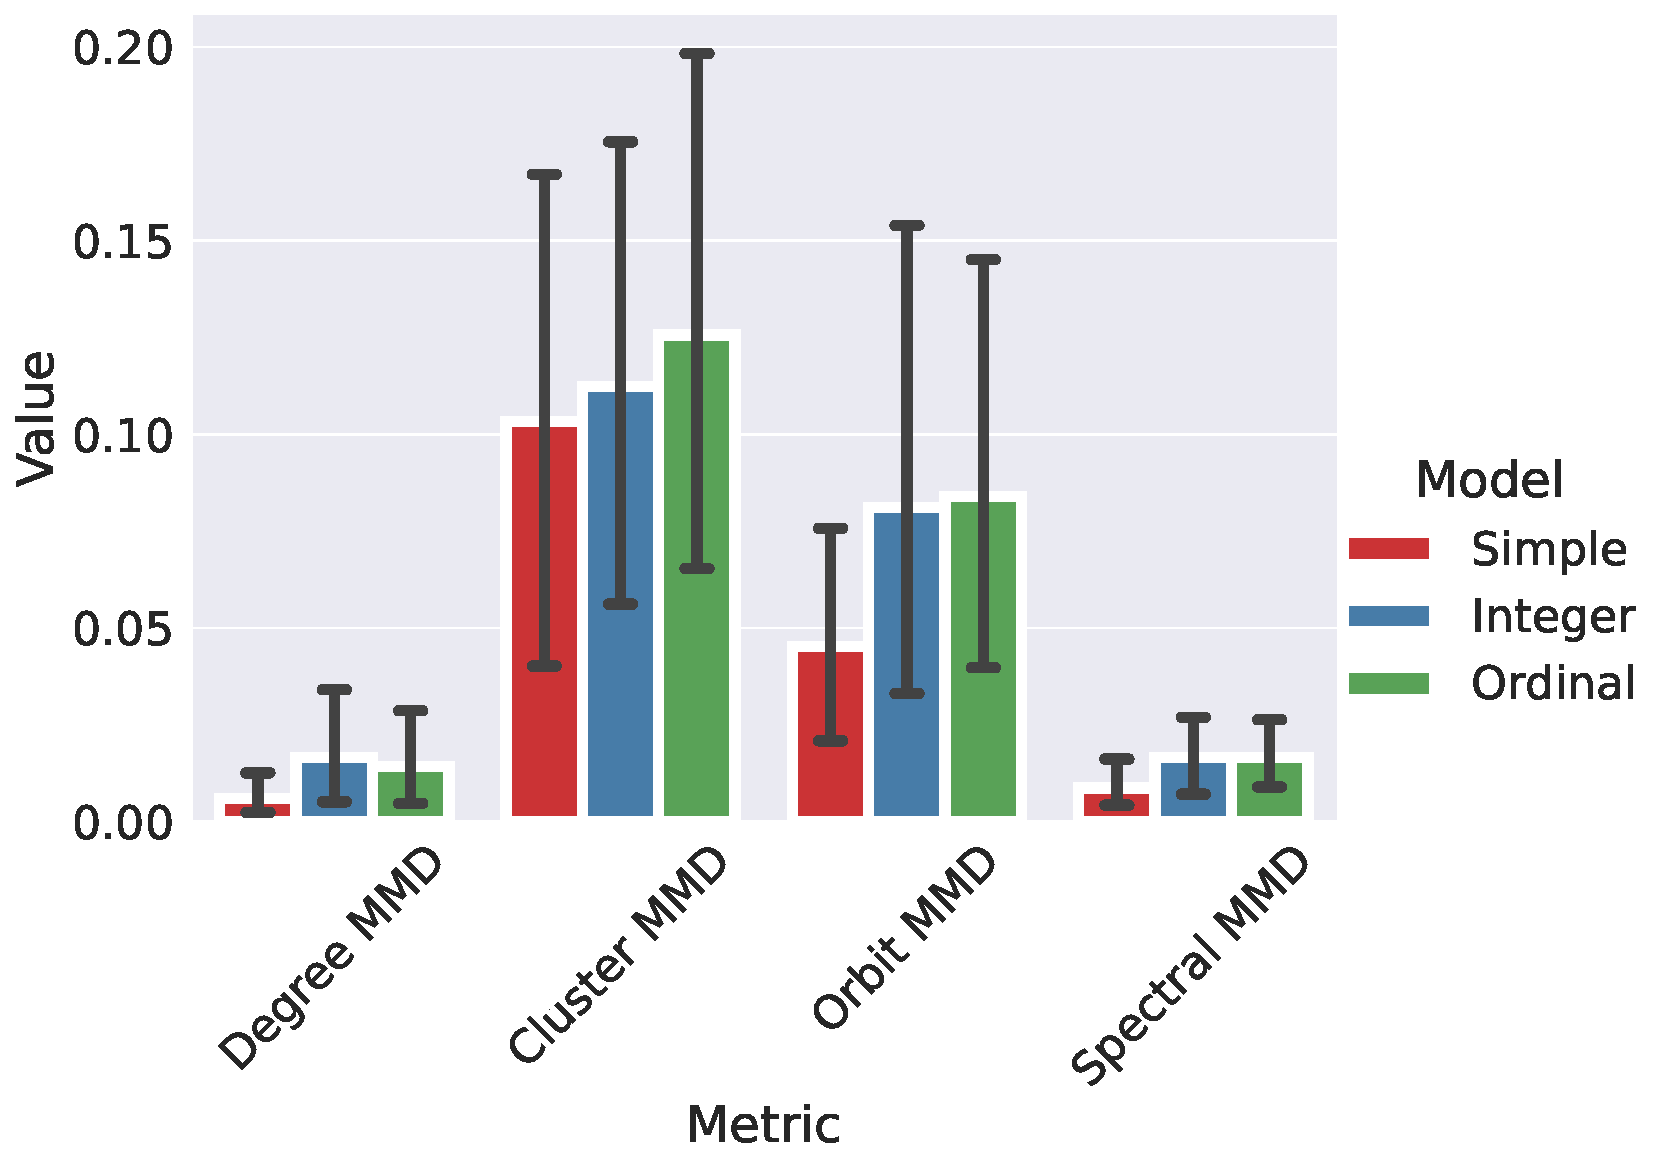
\includegraphics[width=0.475\linewidth]{figures/higendiff/ablation_model.pdf}
    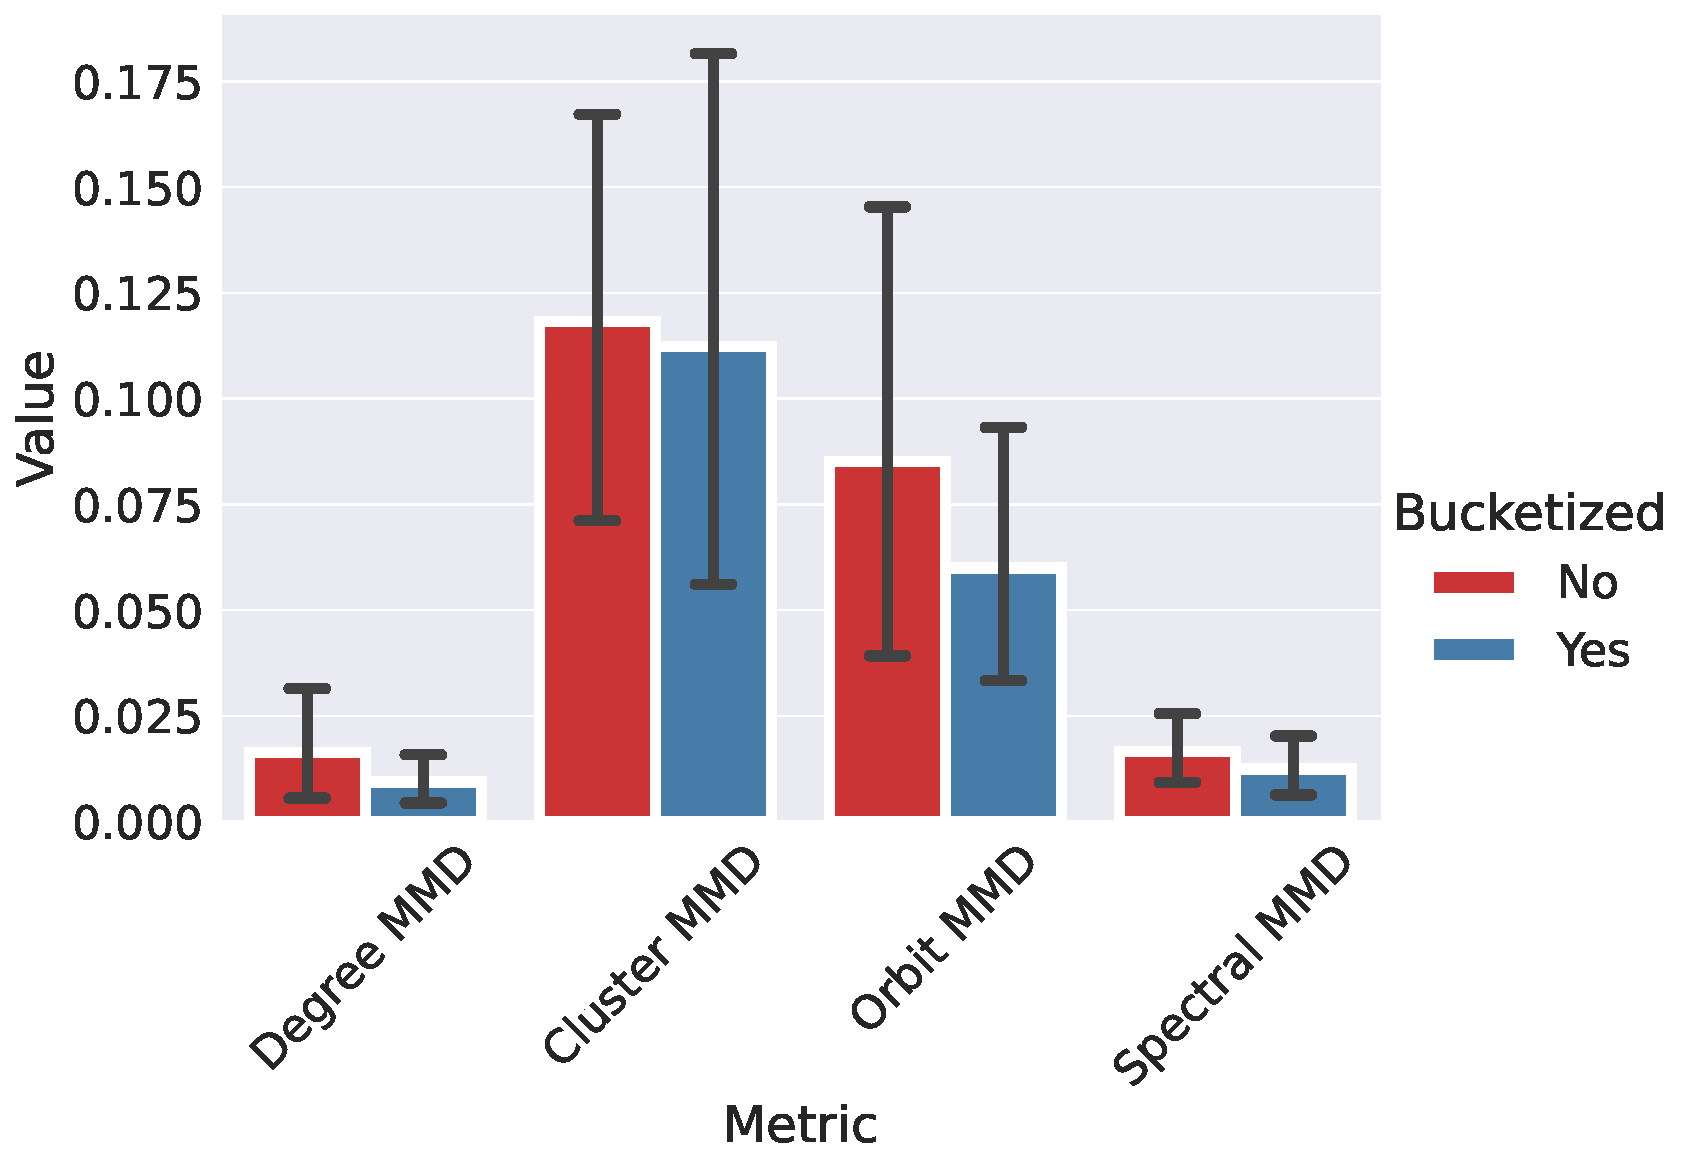
\includegraphics[width=0.475\linewidth]{figures/higendiff/ablation_bucketized.pdf}
    \caption[MMD metric values vs. different HiGenDiff model configurations.]{MMD metric values average across datasets vs. different HiGenDiff model configurations. Left vs right: ablation of the root weight diffusion model vs the effect of bucketization.}
    \label{fig:higendiff_ablation}
\end{figure}

Next, to contextualize our best achieved performance, we provide a comparison to baselines in Table \ref{tab:higendiff_baselines}, namely DiGress \cite{vignac_digress_2022}, the HiGen networks of \cite{karami_higen_2024}, and MRGrad \cite{karami_multi-resolution_2024}. From the comparison table, it is evident that most often HiGenDiff is the top performer. If not, almost surely the second best, and this is most prominent with the DD2 dataset, where, although HiGen is still unbeatable, the best results of HiGenDiff are much more competitive than those of MRGrad. Observe also that the Naive HiGenDiff learning setup also ranks decently high among the competition.

\begin{table}[H]
    \caption[Best HiGenDiff MMDs compared to previous baselines.]{Best HiGenDiff MMDs compared to previous baselines (lower is better). The metric value for the best model for each metric is highlighted in bold font, while the second best is underlined. Credit to \cite{karami_multi-resolution_2024} for most of the values.}
    \label{tab:higendiff_baselines}
    \centering
    \begin{tabular}{llrrrr}
    \toprule
       Dataset & Model & Degree & Cluster & Orbit & Spectral \\
    \midrule
       enzyme  & DiGress  & \underline{0.0040} & 0.0830 & \underline{0.0020} & \textemdash \\
       enzyme  & HiGen  & 0.0120 & 0.0380 & \textbf{0.0007} & \textemdash \\
       enzyme  & MRGrad  & 0.0064 & 0.0653 & 0.0047 &  0.0590 \\
       enzyme  & HiGenDiff-Naive  & 0.0297 & \underline{0.0243} & 0.0059 & \underline{0.0227} \\
       enzyme  & HiGenDiff-Best & \textbf{0.0020} & \textbf{0.0160} & 0.0250 & \textbf{0.0050} \\
    \midrule
       SBM  & DiGress  & \underline{0.0013} & 0.0498 & 0.0433 & \textemdash \\
       SBM  & HiGen  & 0.0019 & 0.0498 & \textbf{0.0352} & \underline{0.0046} \\
       SBM  & MRGrad  & 0.0381 & \textbf{0.0126} & 0.0446 & 0.0532 \\
       SBM  & HiGenDiff-Naive  & 0.0017 & 0.0298 & 0.0482 & 0.0049 \\
       SBM  & HiGenDiff-Best  & \textbf{0.0010} & \underline{0.0270} & \underline{0.0400} & \textbf{0.0040} \\
    \midrule
       Ego2  & DiGress  & 0.0708  & \underline{0.0092} & 0.1205 & \textemdash \\
       Ego2  & HiGen  & \underline{0.0472} & \textbf{0.0031} & \underline{0.0387} &  \textemdash  \\
       Ego2  & MRGrad  & 0.2150  & 0.0410  & 0.0609 & \underline{0.0425}  \\
       Ego2  & HiGenDiff-Best  & \textbf{0.0020} & 0.0550 & \textbf{0.0330} & \textbf{0.0030} \\
    \midrule
       DD2  & HiGen  & \textbf{0.0012} & \textbf{0.0435} & \textbf{0.0234} & \textbf{0.0025} \\
       DD2  & MRGrad  & 0.1250 & 1.0473 & 0.2771 & 0.1561 \\
       DD2  & HiGenDiff-Best & \underline{0.0020} & \underline{0.0720} & \underline{0.0240} & \underline{0.0050} \\
    \bottomrule
    \end{tabular}
\end{table}

Before concluding, we provide visual examples from the graph datasets in Figure \ref{fig:higendiff_examples}. An appearance-based comparison also verifies the generally high quality of artificially generated hierarchical graph structures. 

\begin{figure}[H]
    \centering
    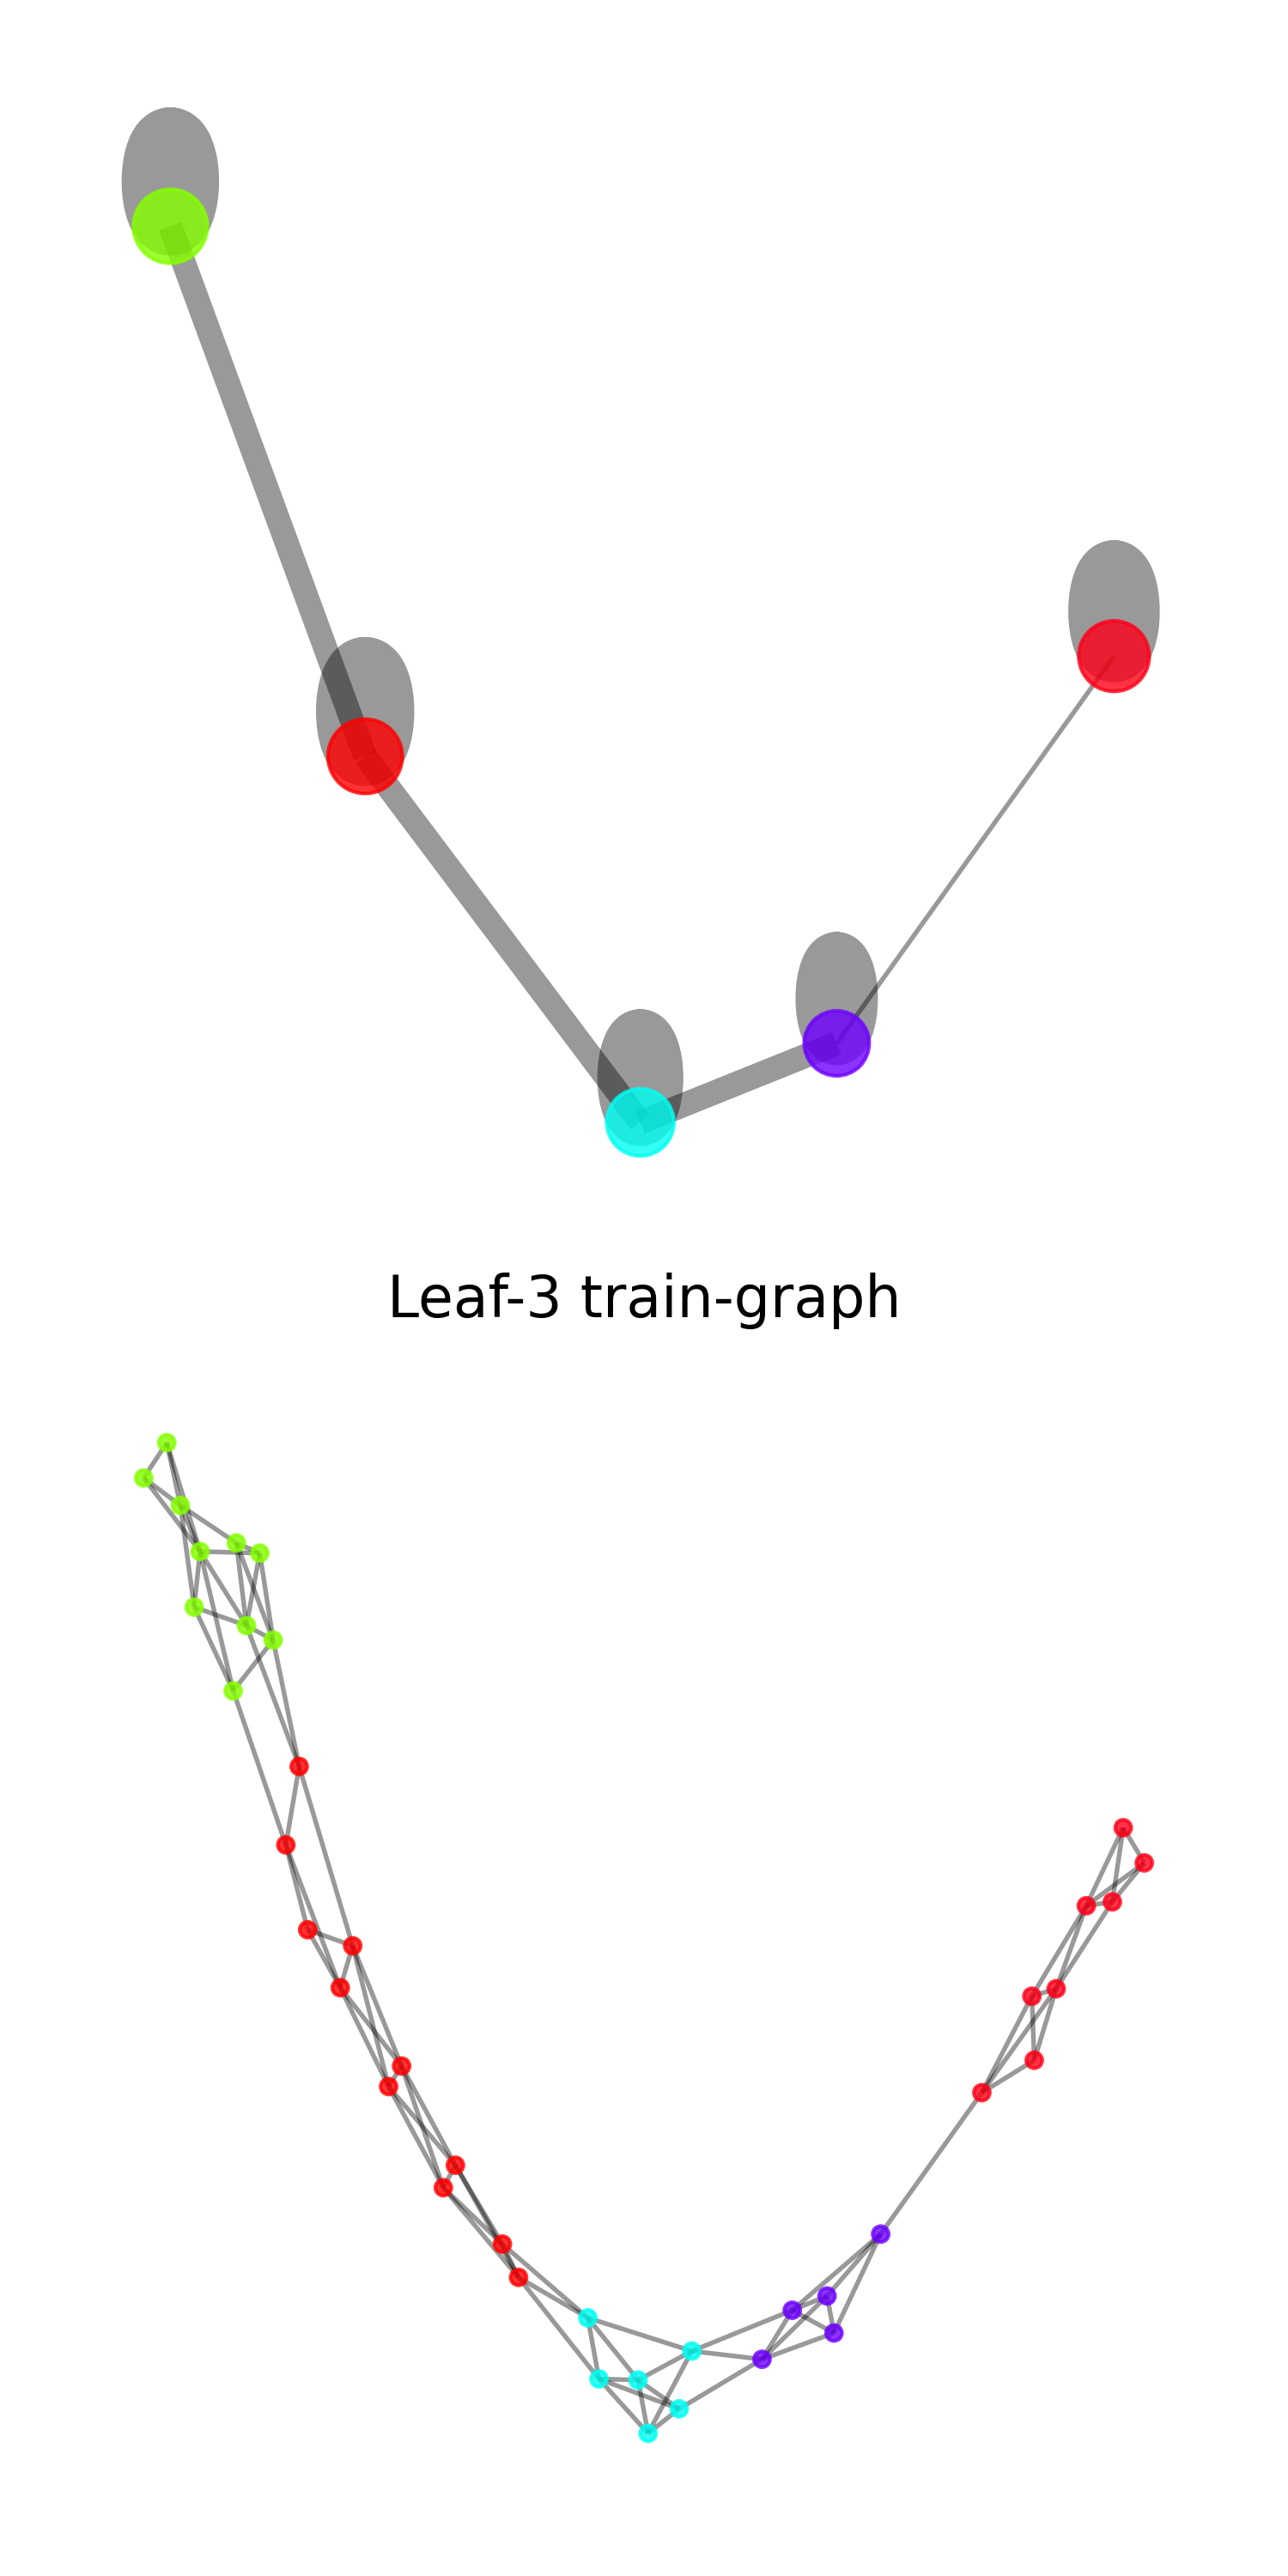
\includegraphics[width=0.15\linewidth]{figures/higendiff/enzyme_true.png}
    \hfill
    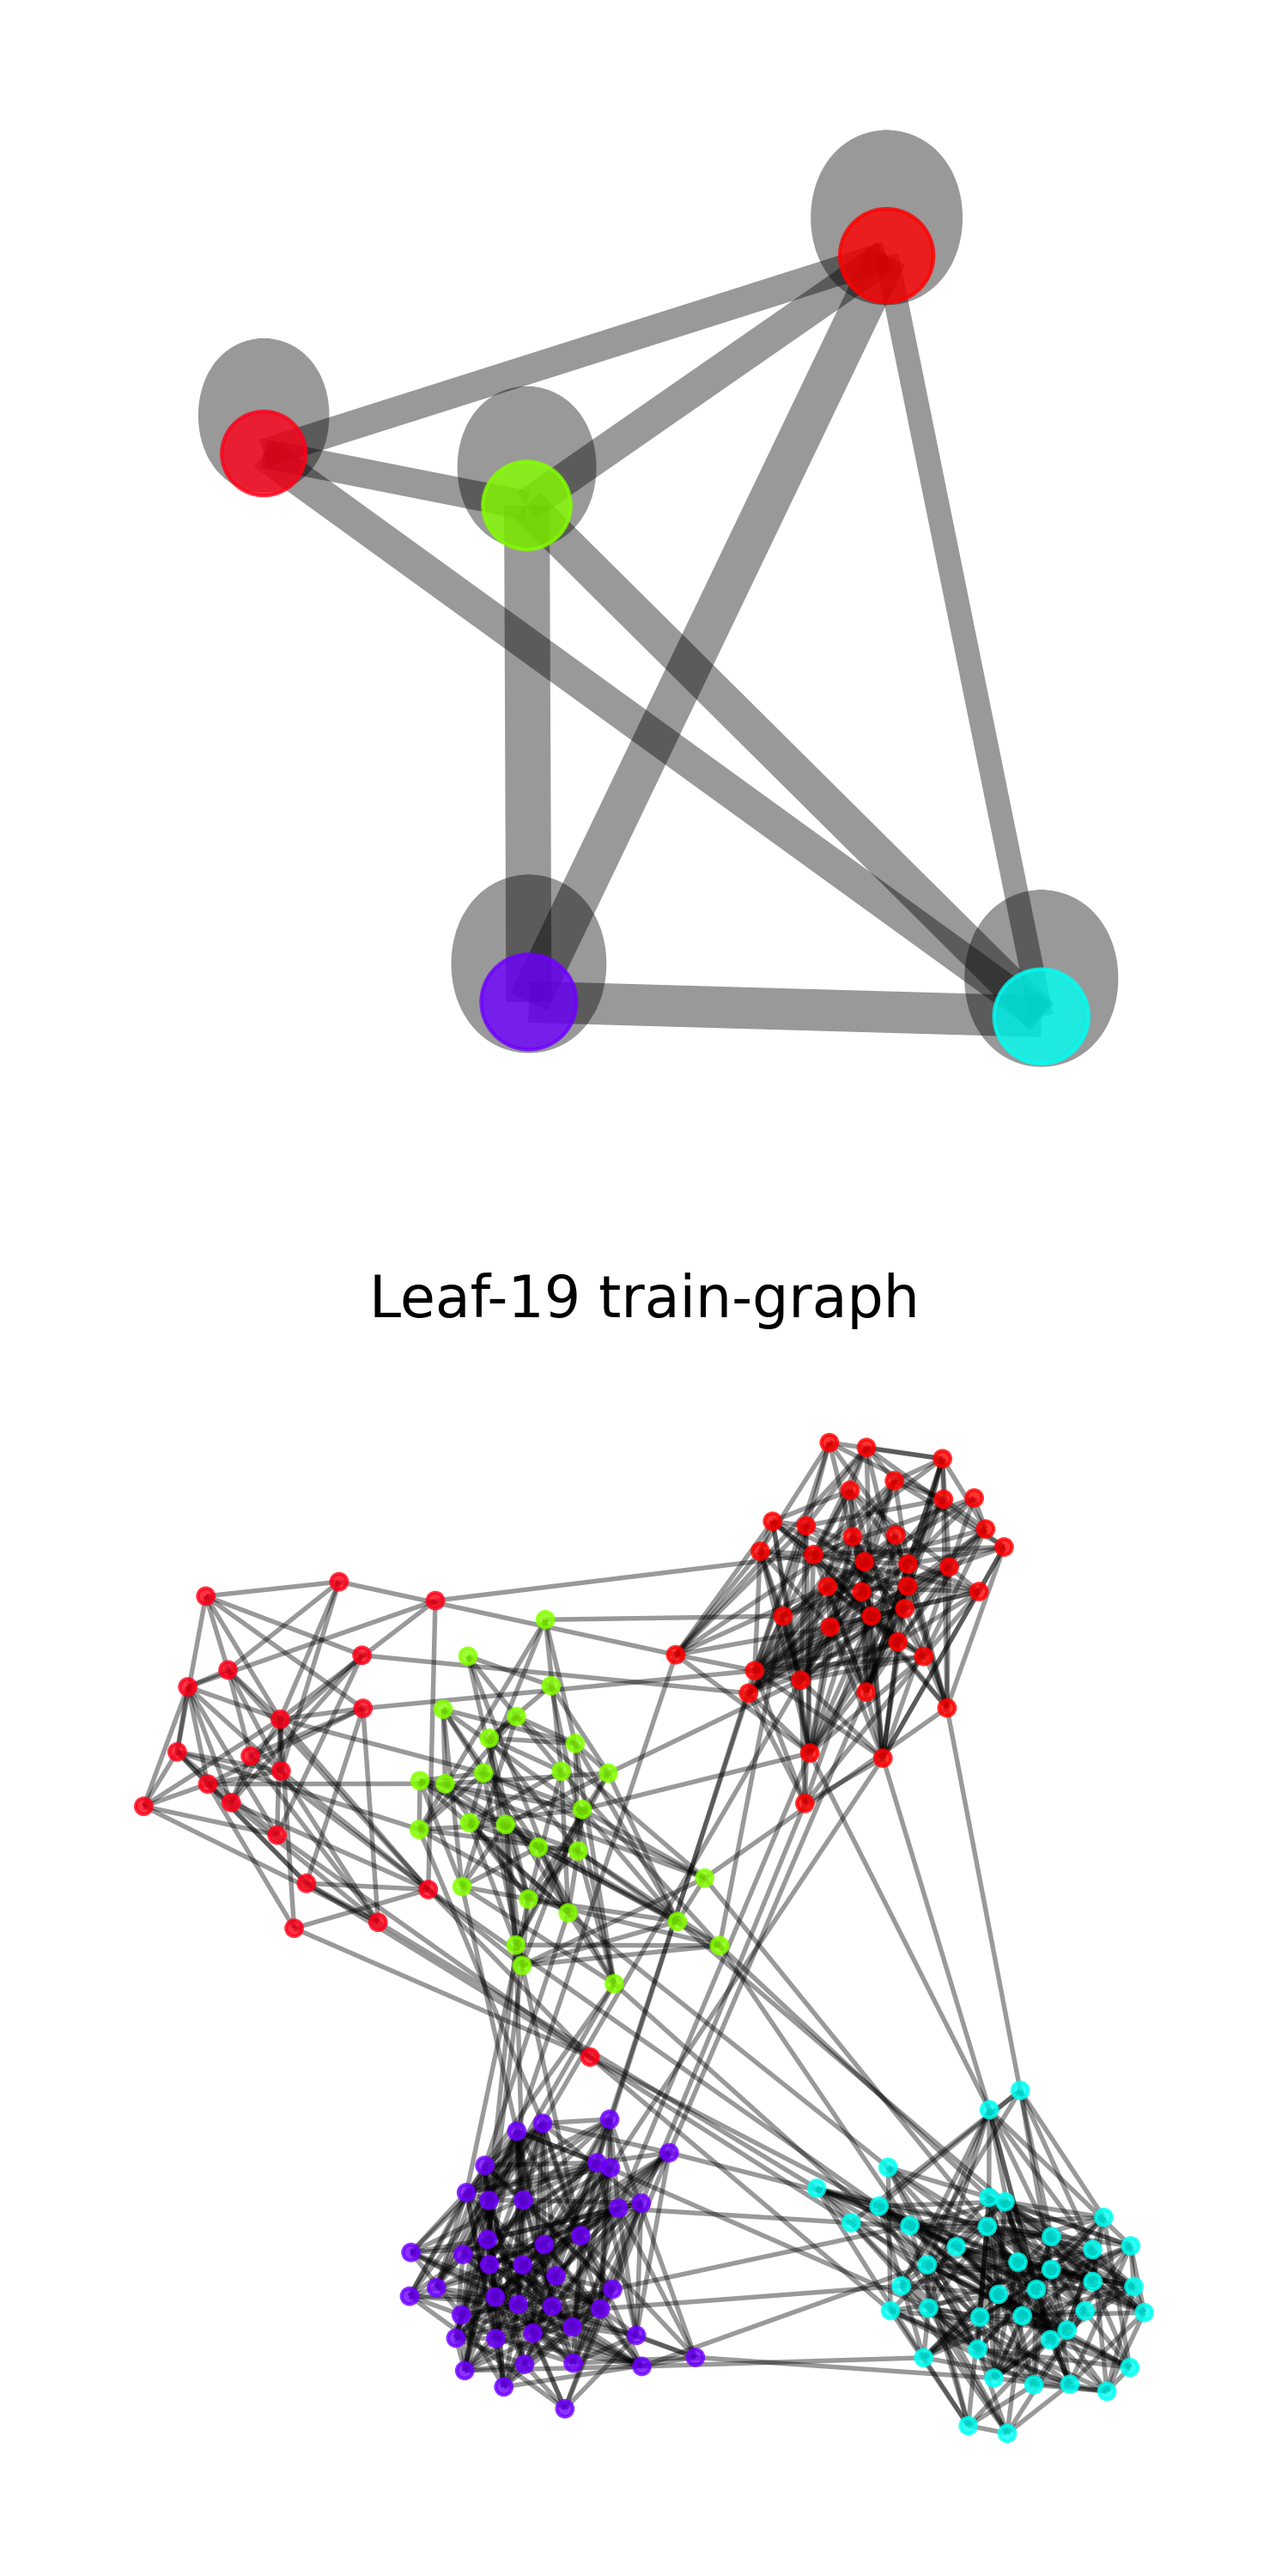
\includegraphics[width=0.15\linewidth]{figures/higendiff/sbm_true.png}
        \hfill
    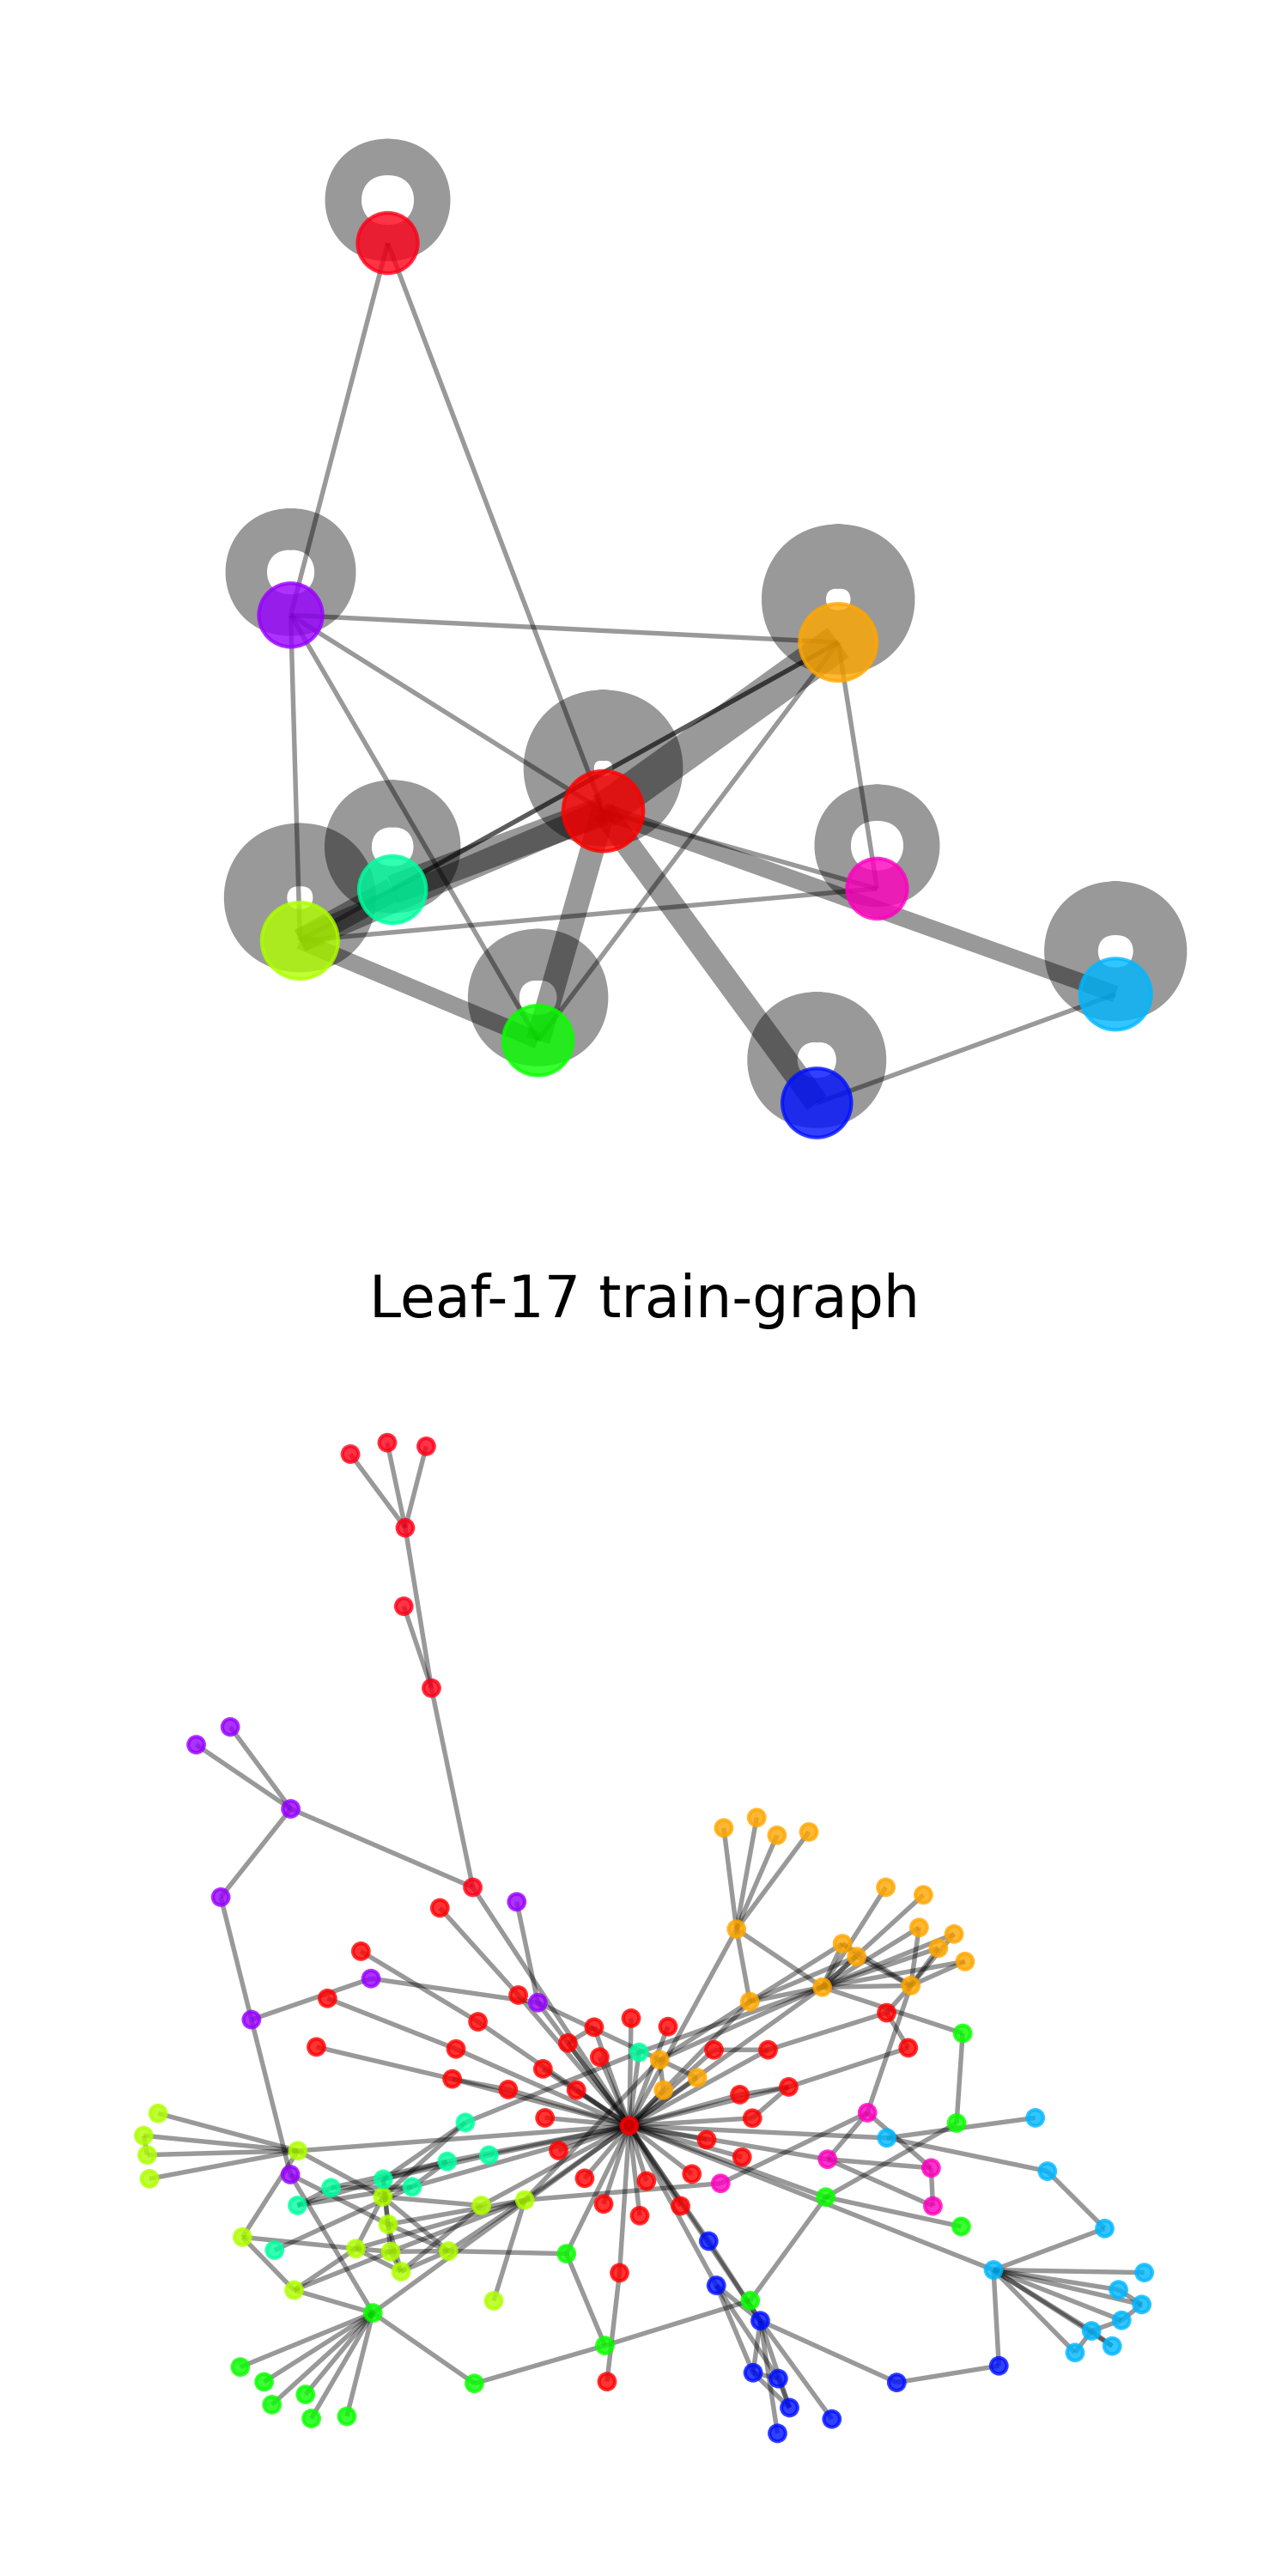
\includegraphics[width=0.15\linewidth]{figures/higendiff/ego2_true.png}
        \hfill
    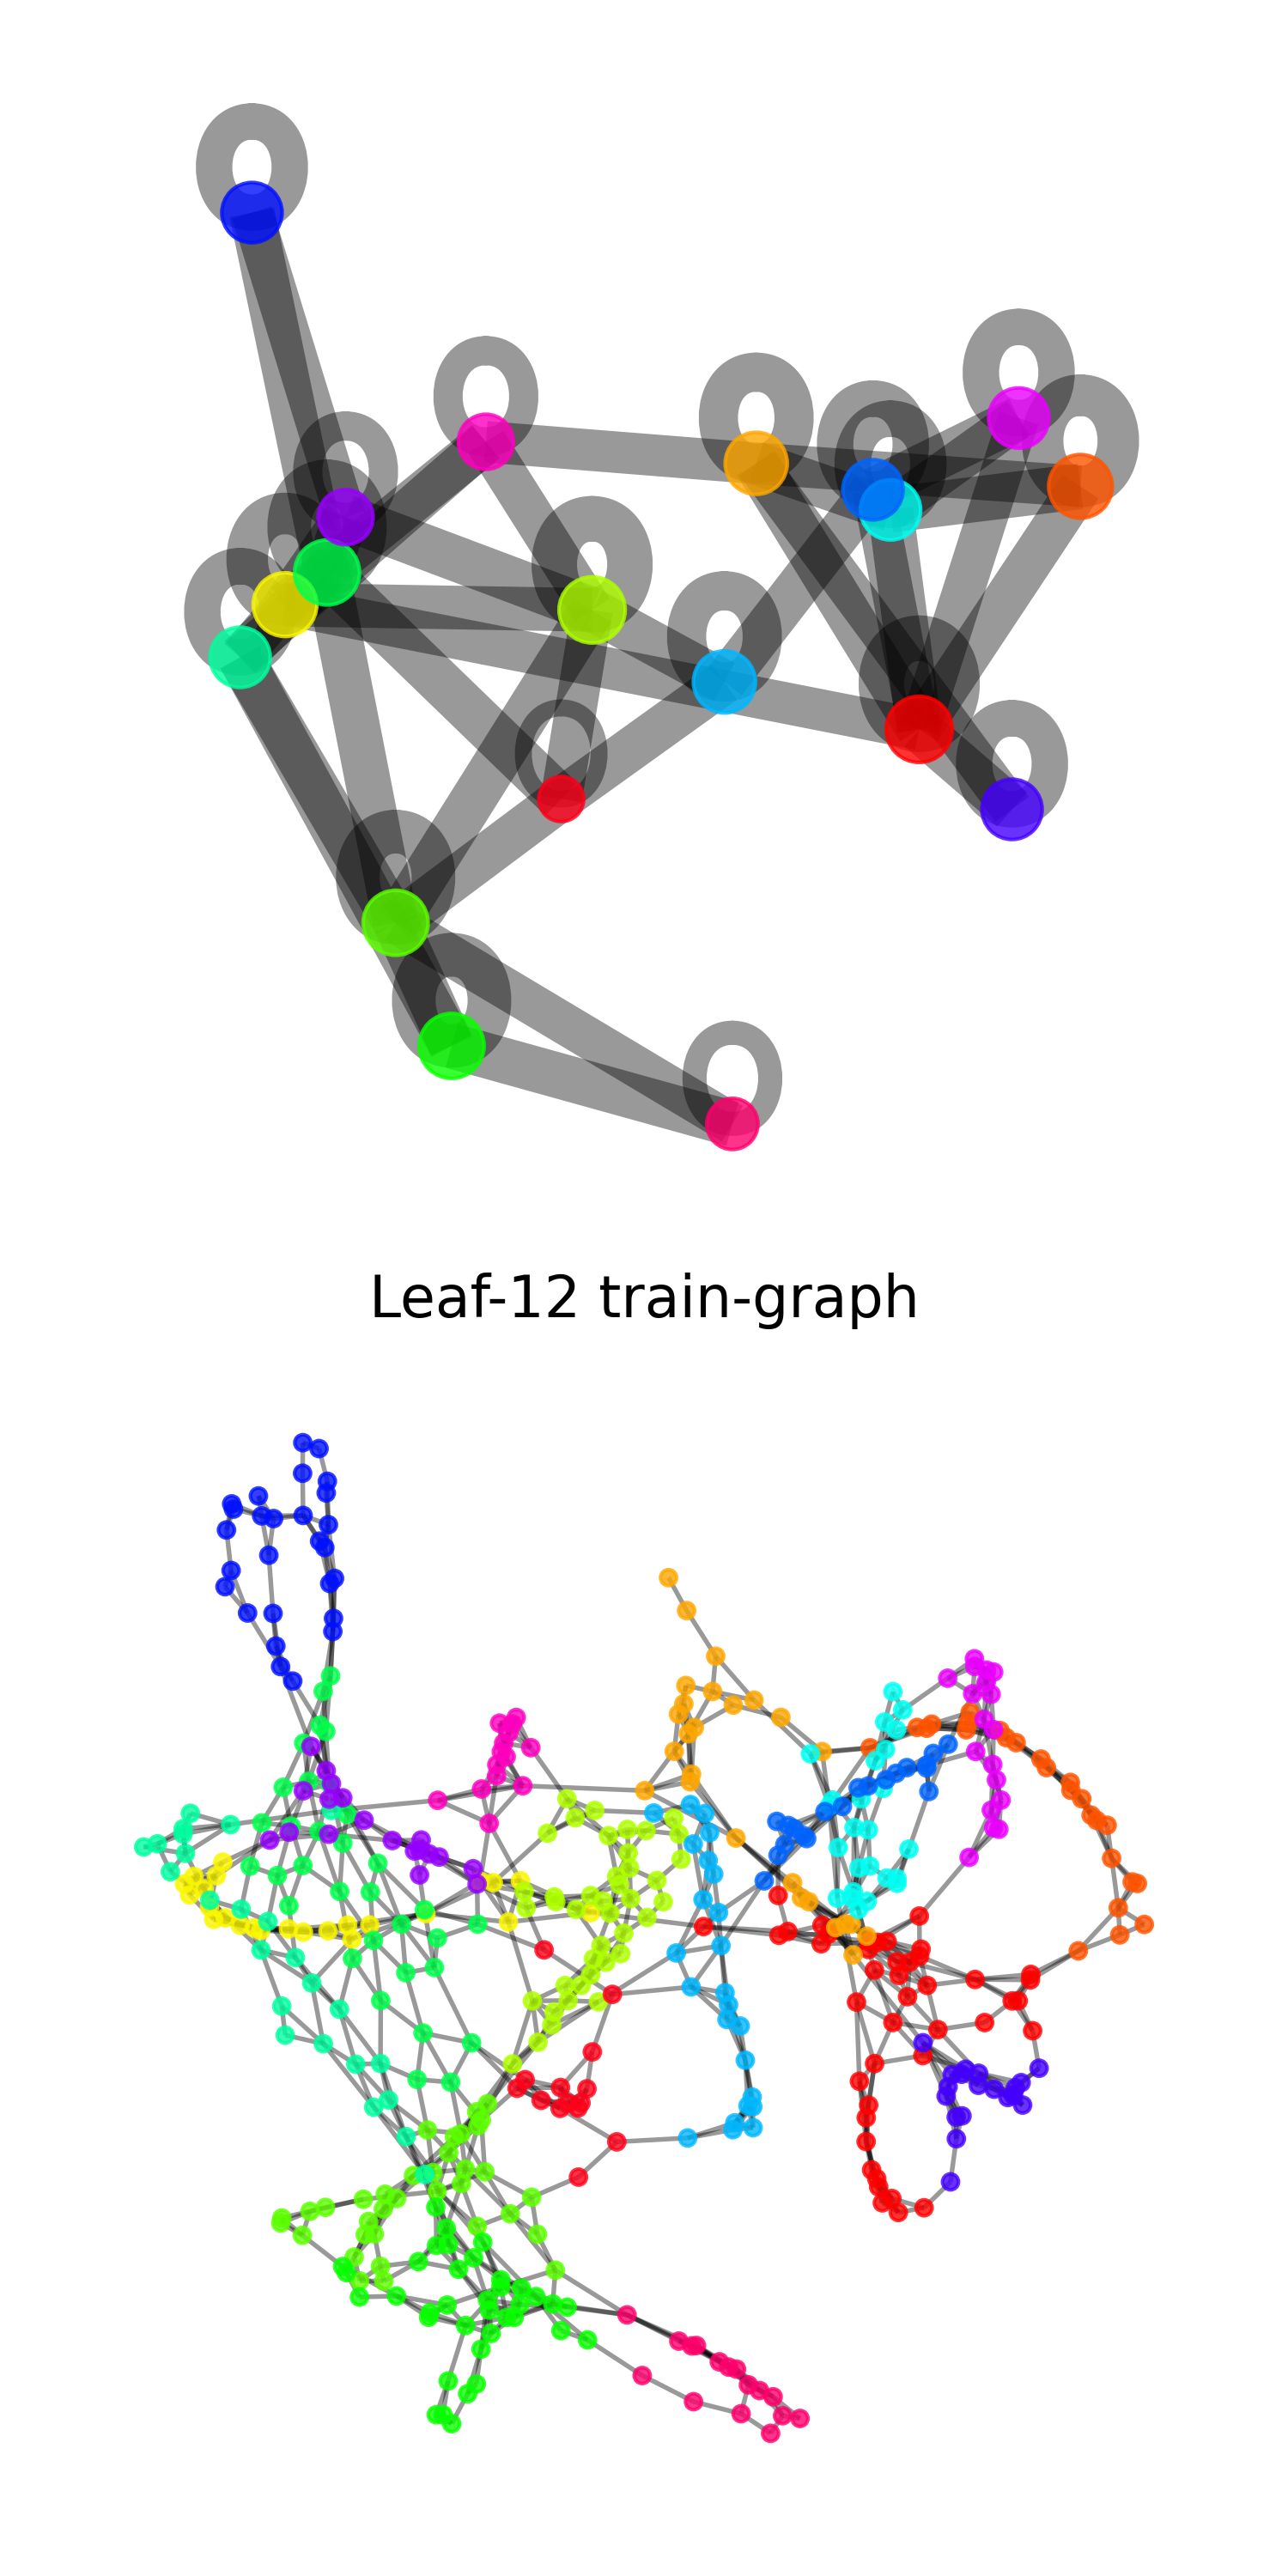
\includegraphics[width=0.15\linewidth]{figures/higendiff/dd2_true.png}
        \hfill
    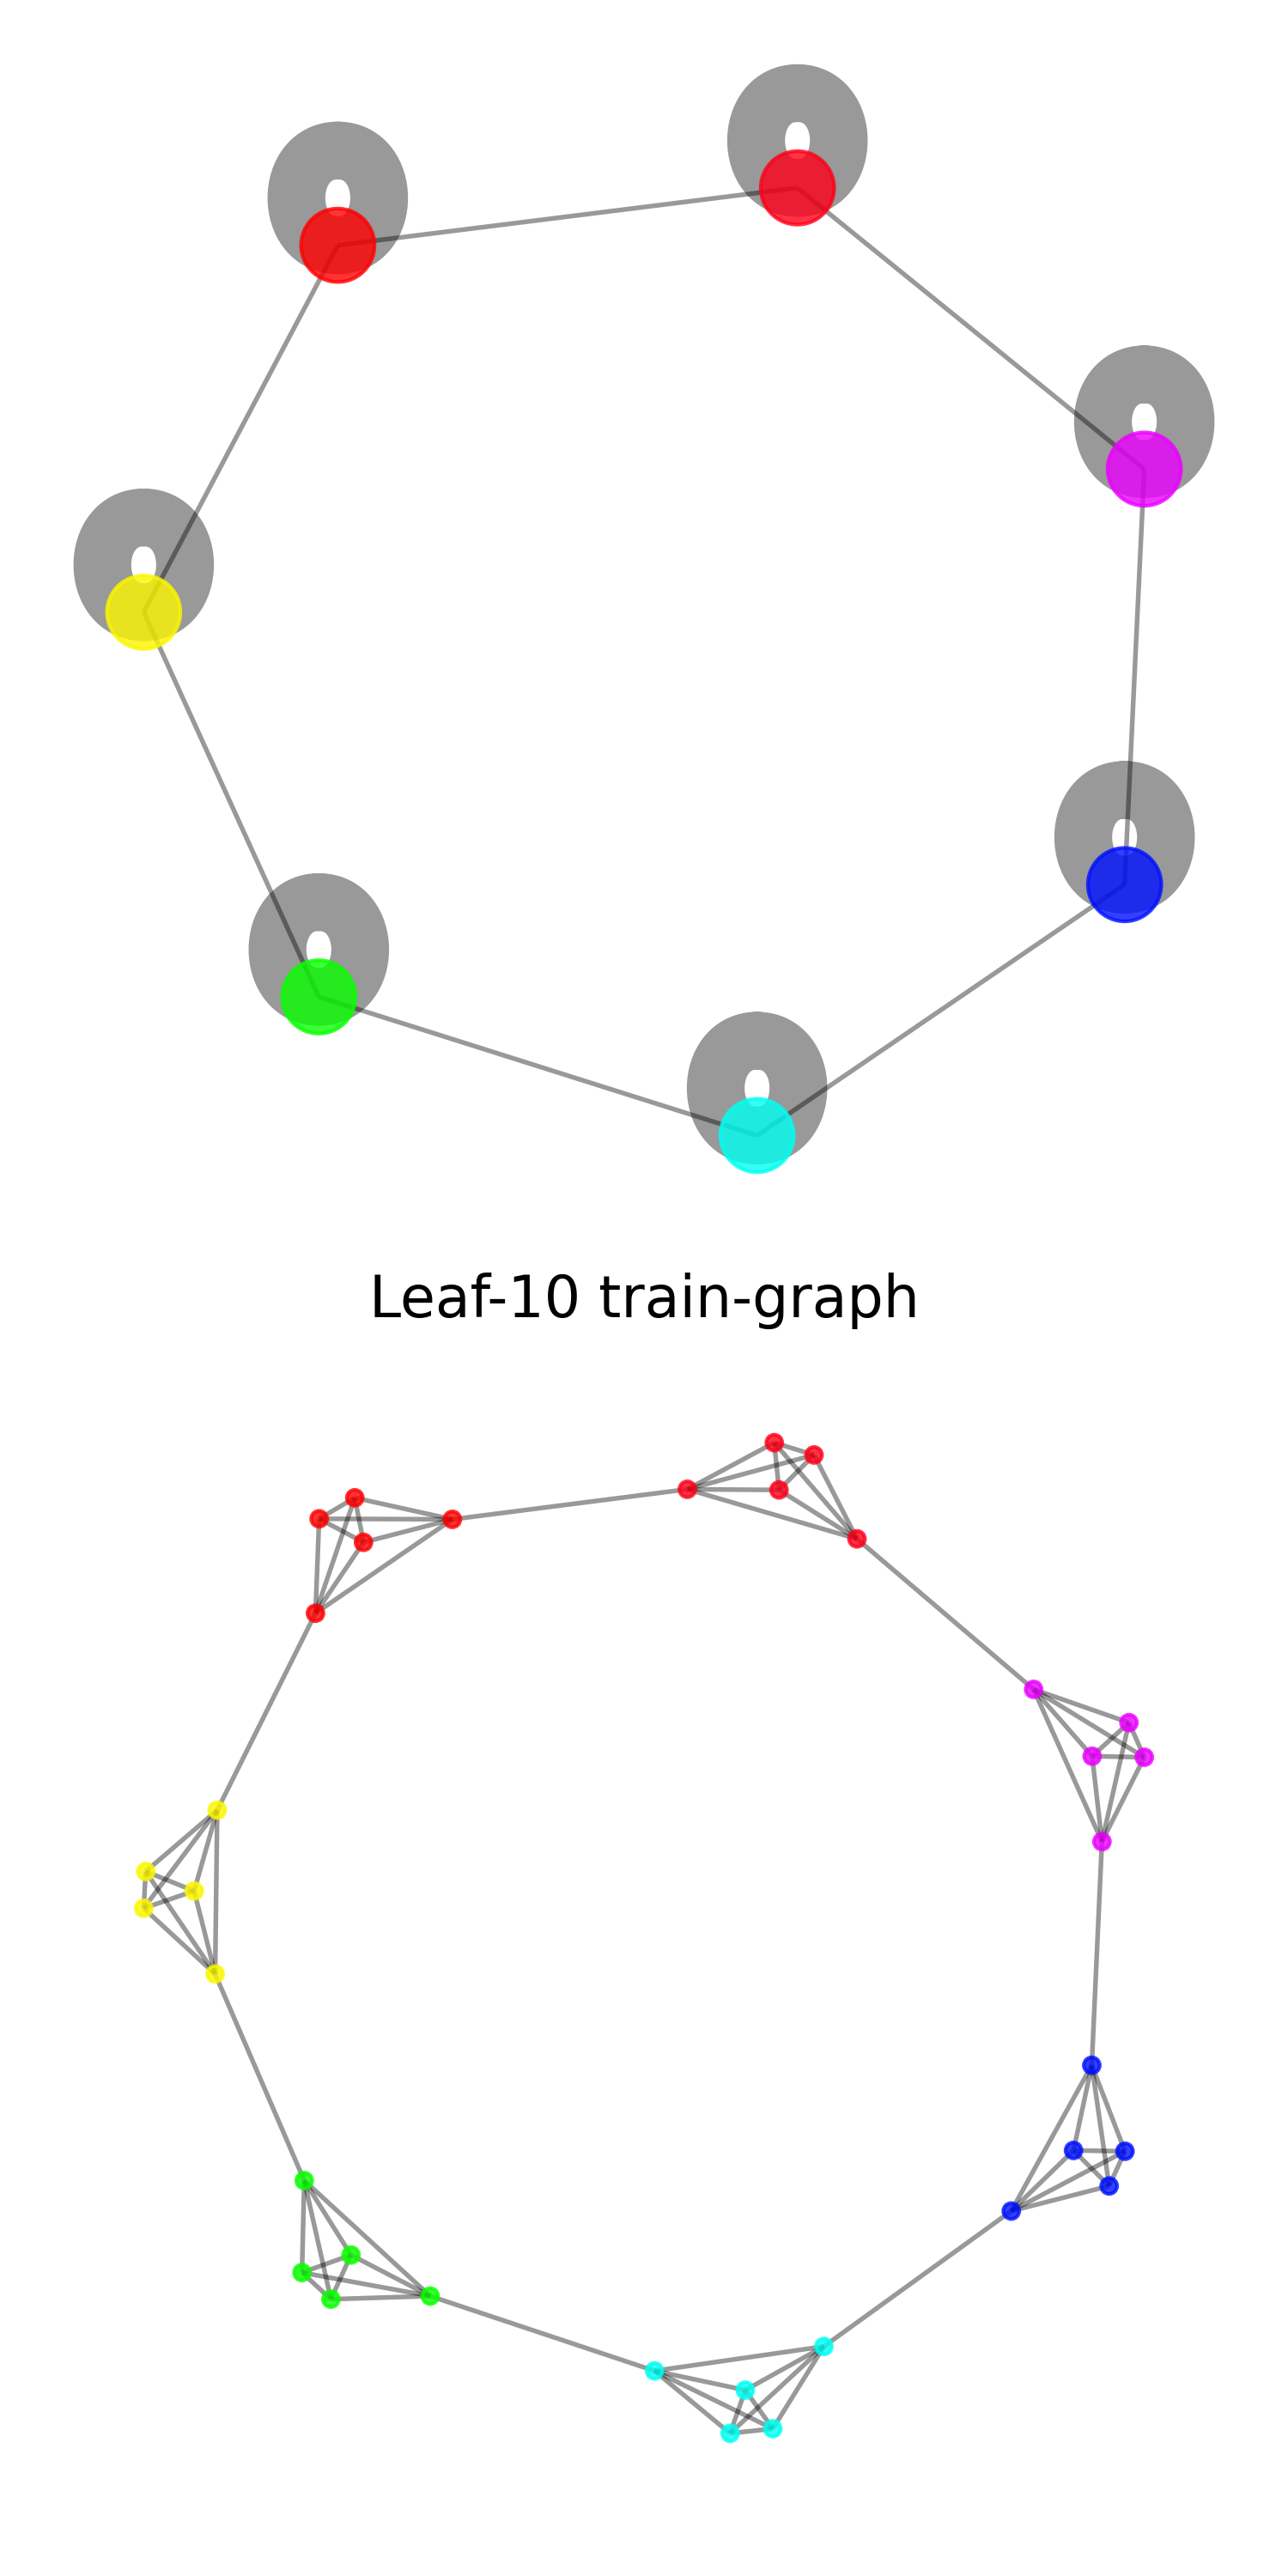
\includegraphics[width=0.15\linewidth]{figures/higendiff/roc_true.png}
        \hfill
    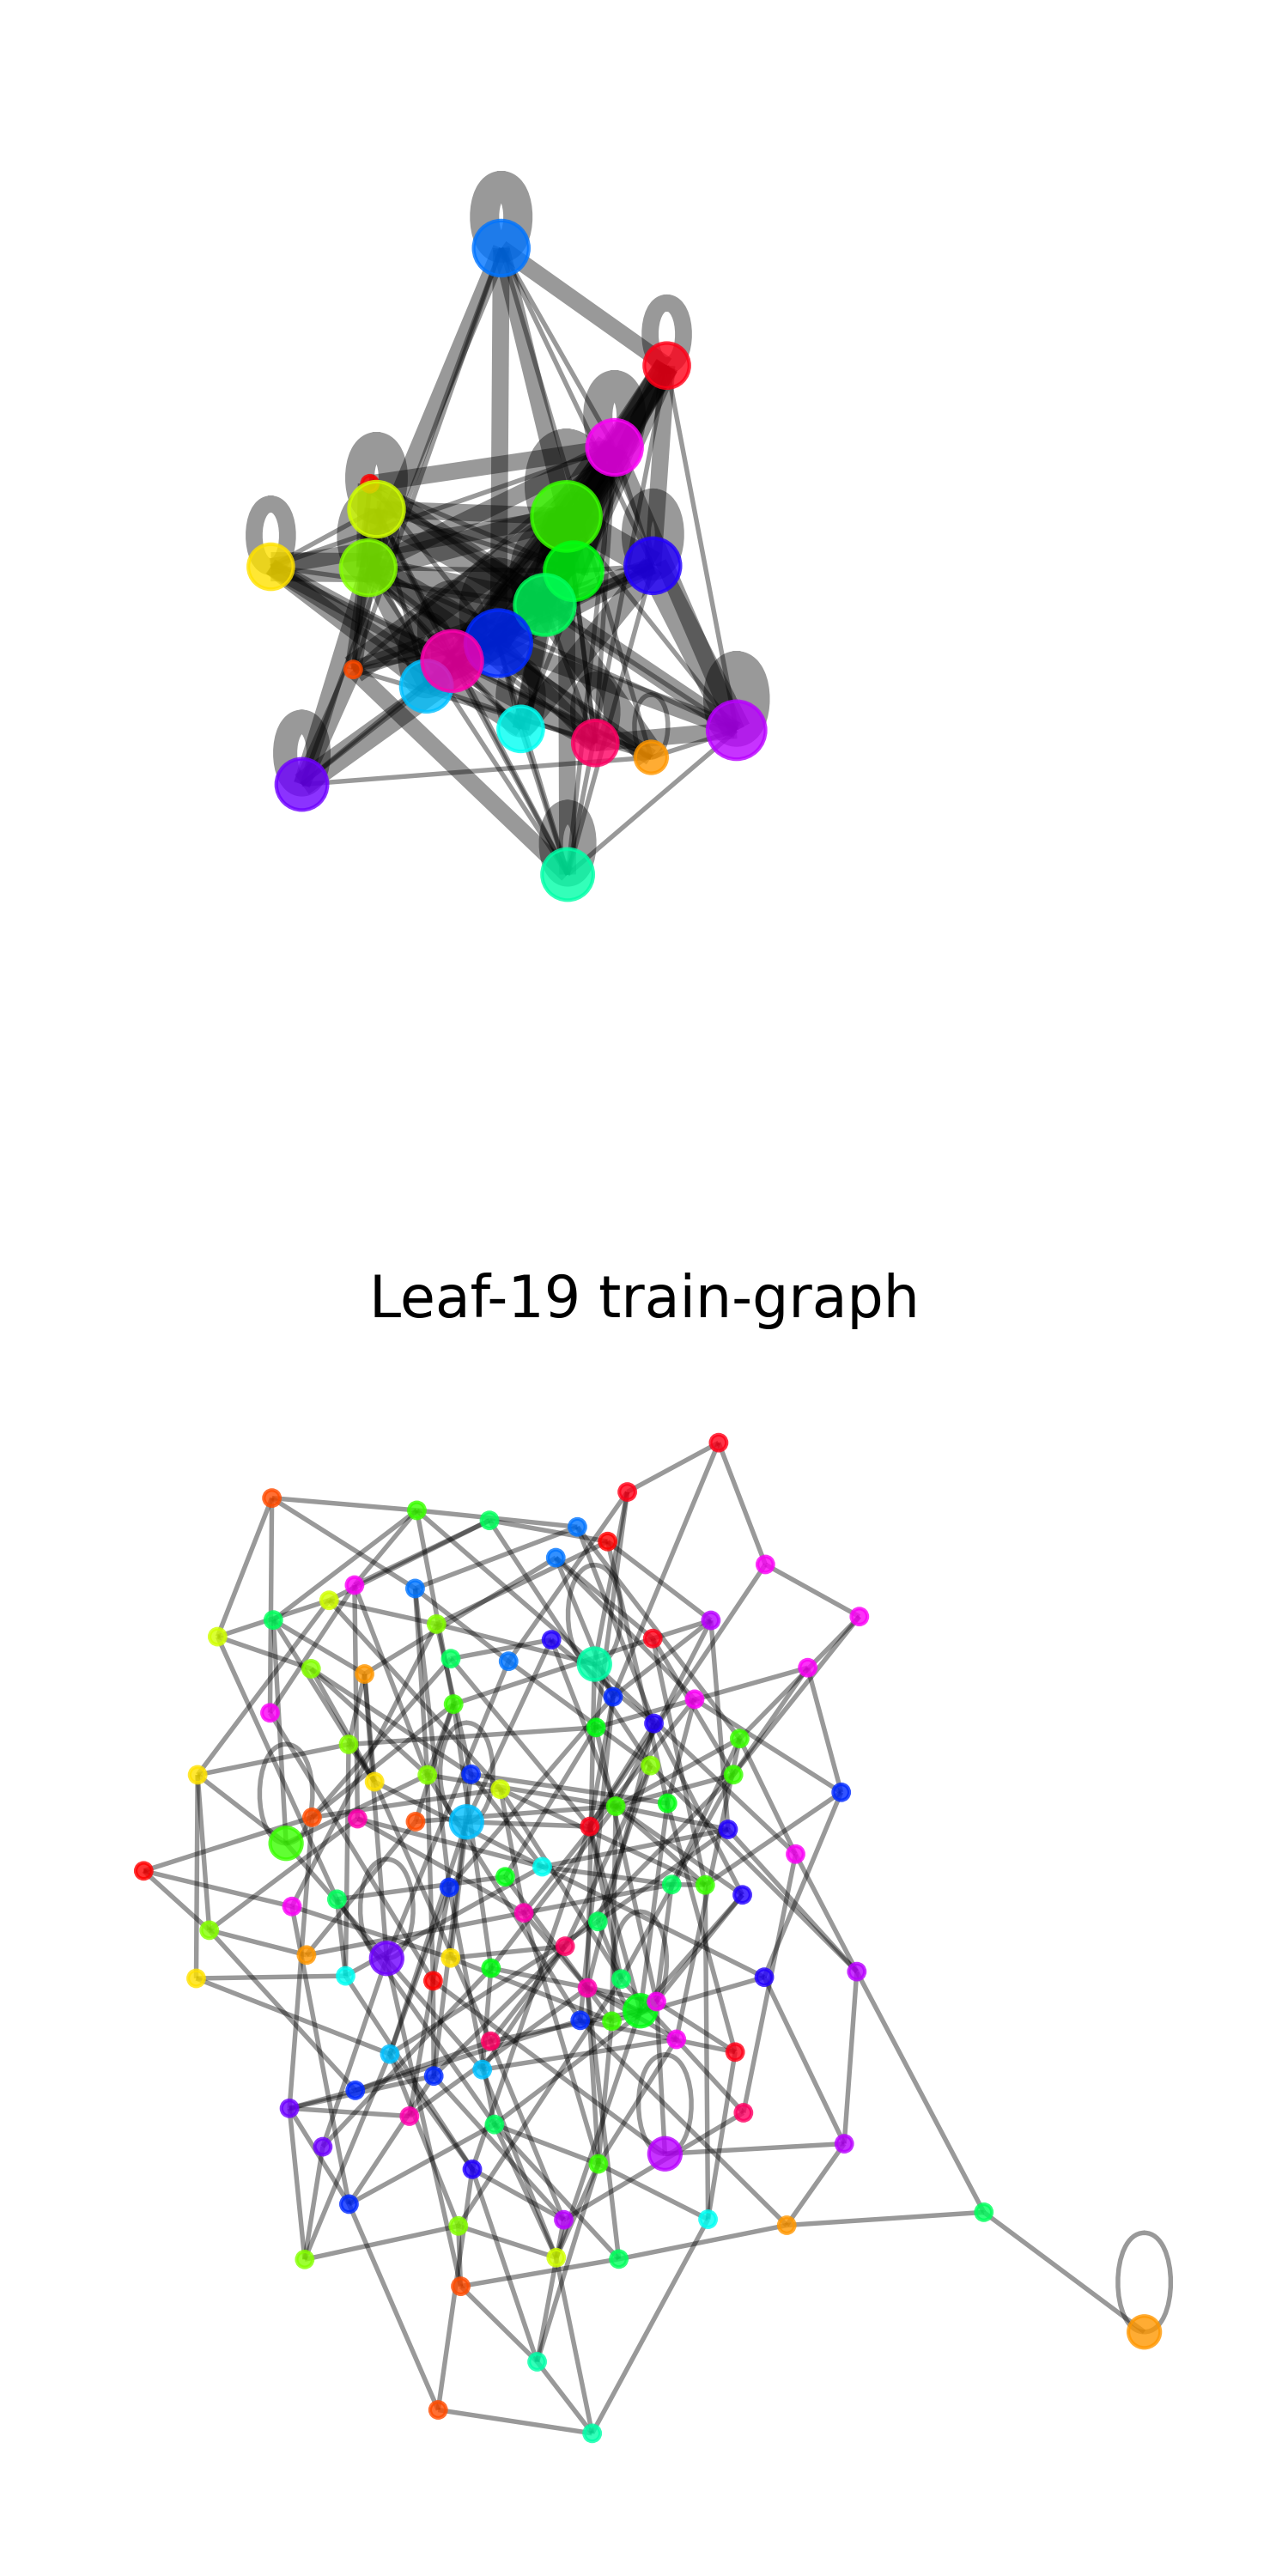
\includegraphics[width=0.15\linewidth]{figures/higendiff/lfr_true.png}
    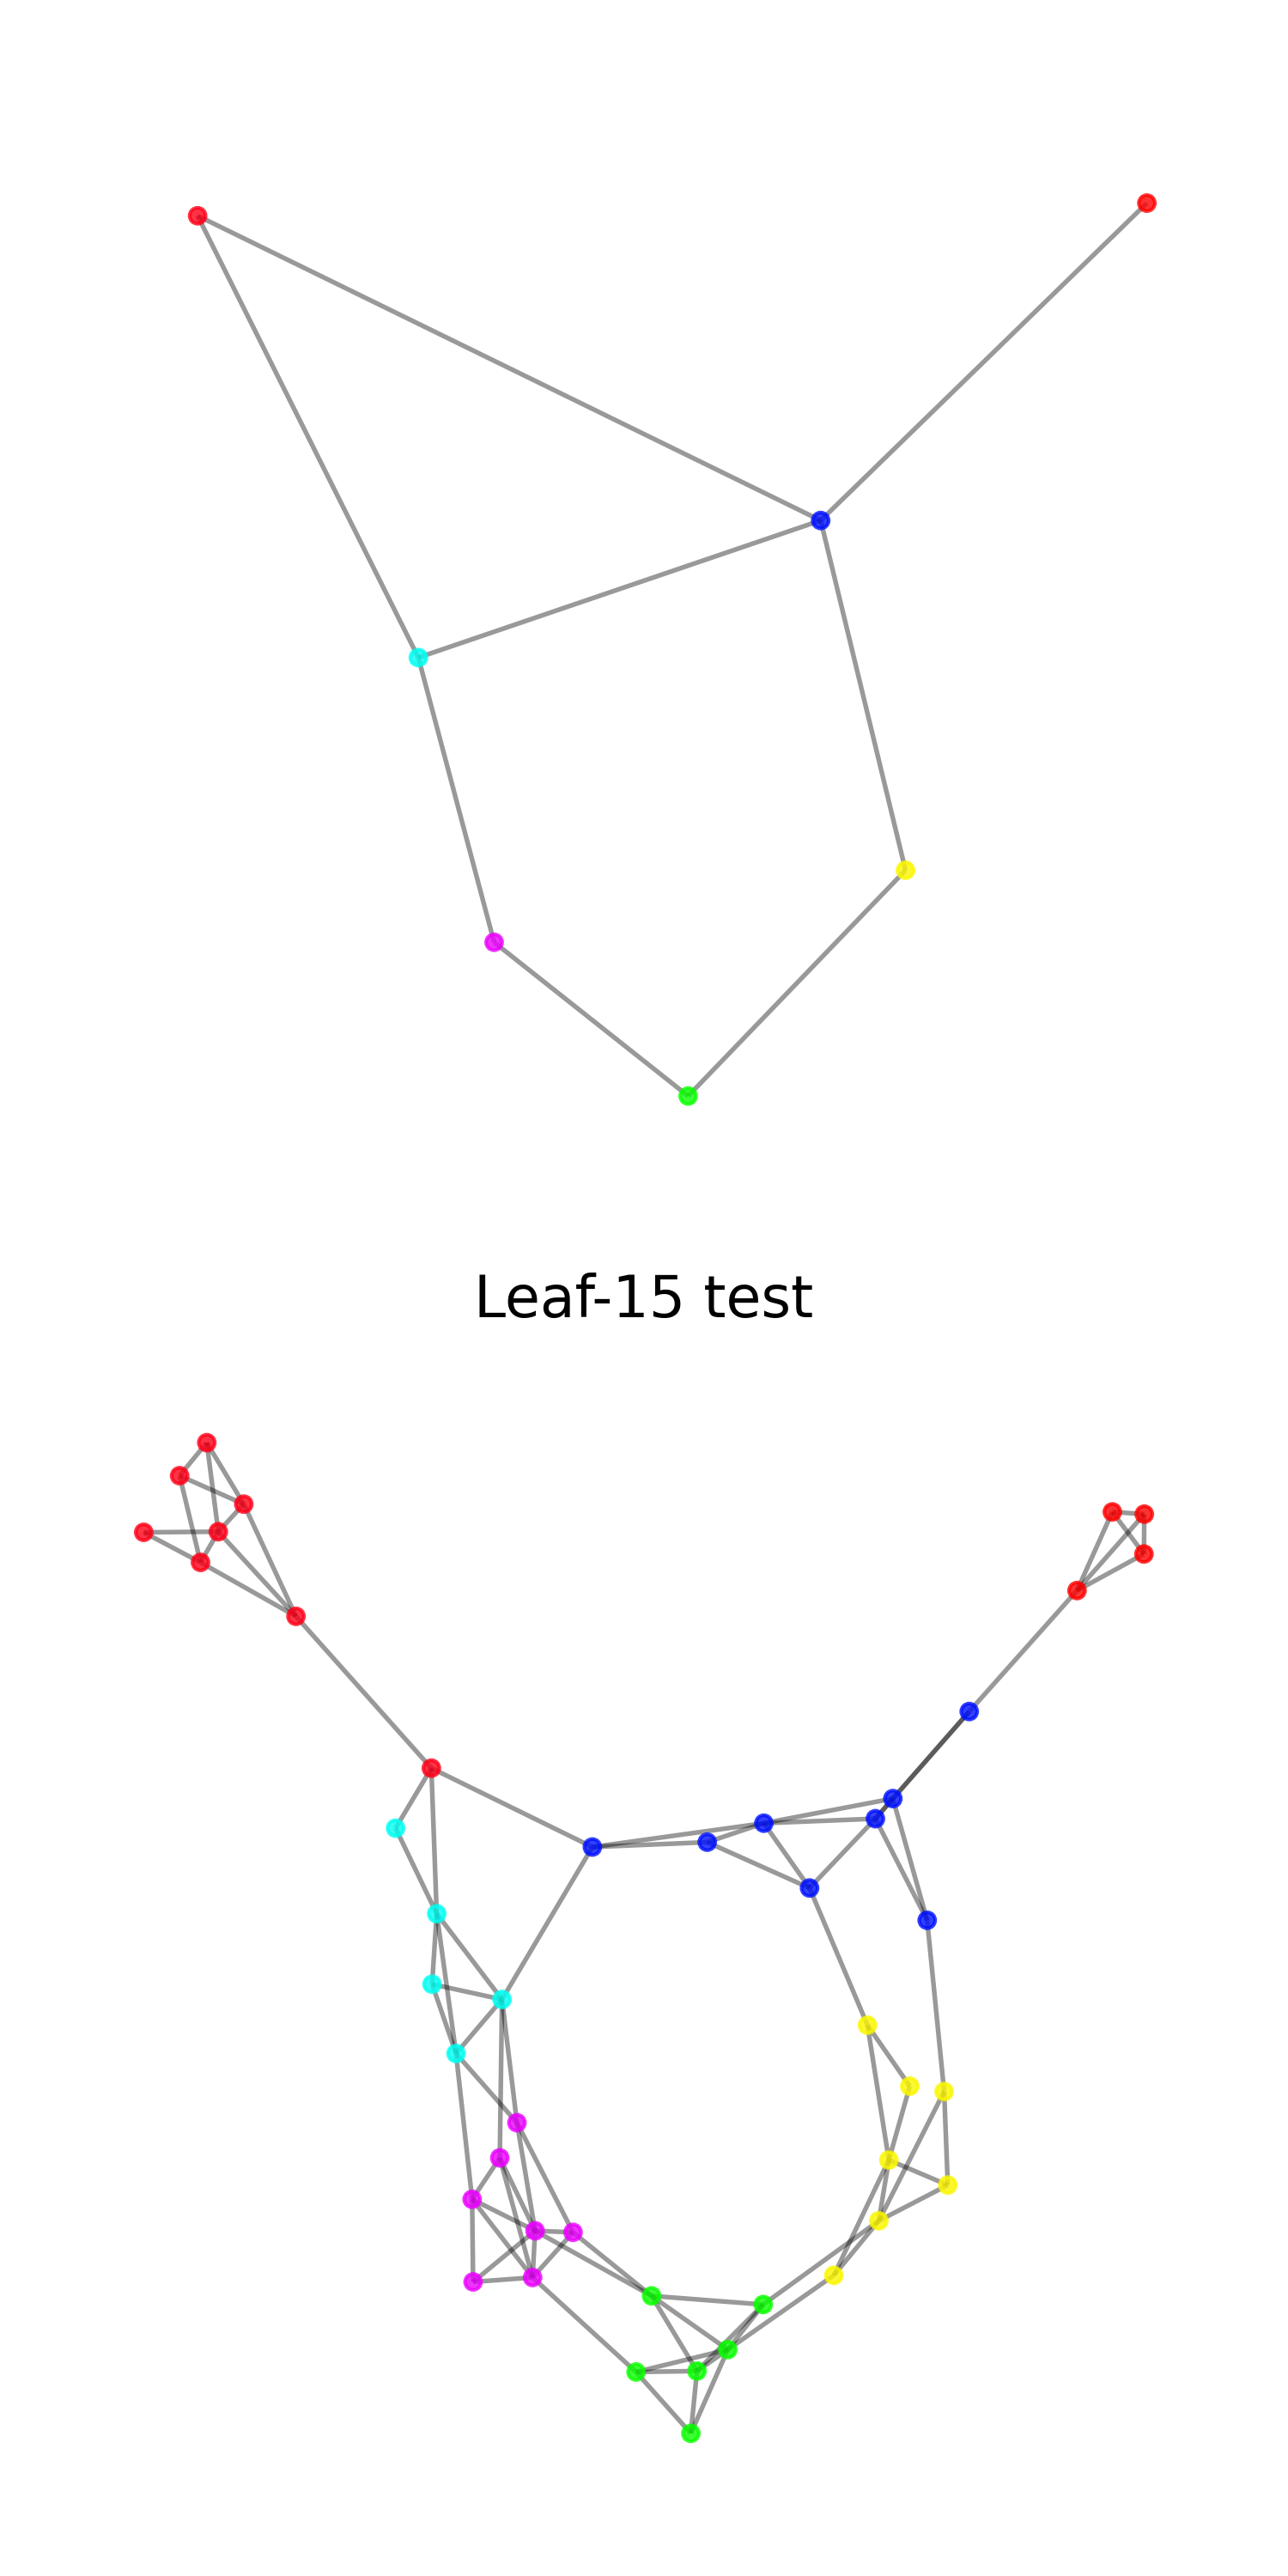
\includegraphics[width=0.15\linewidth]{figures/higendiff/enzyme_gen.png}
    \hfill
    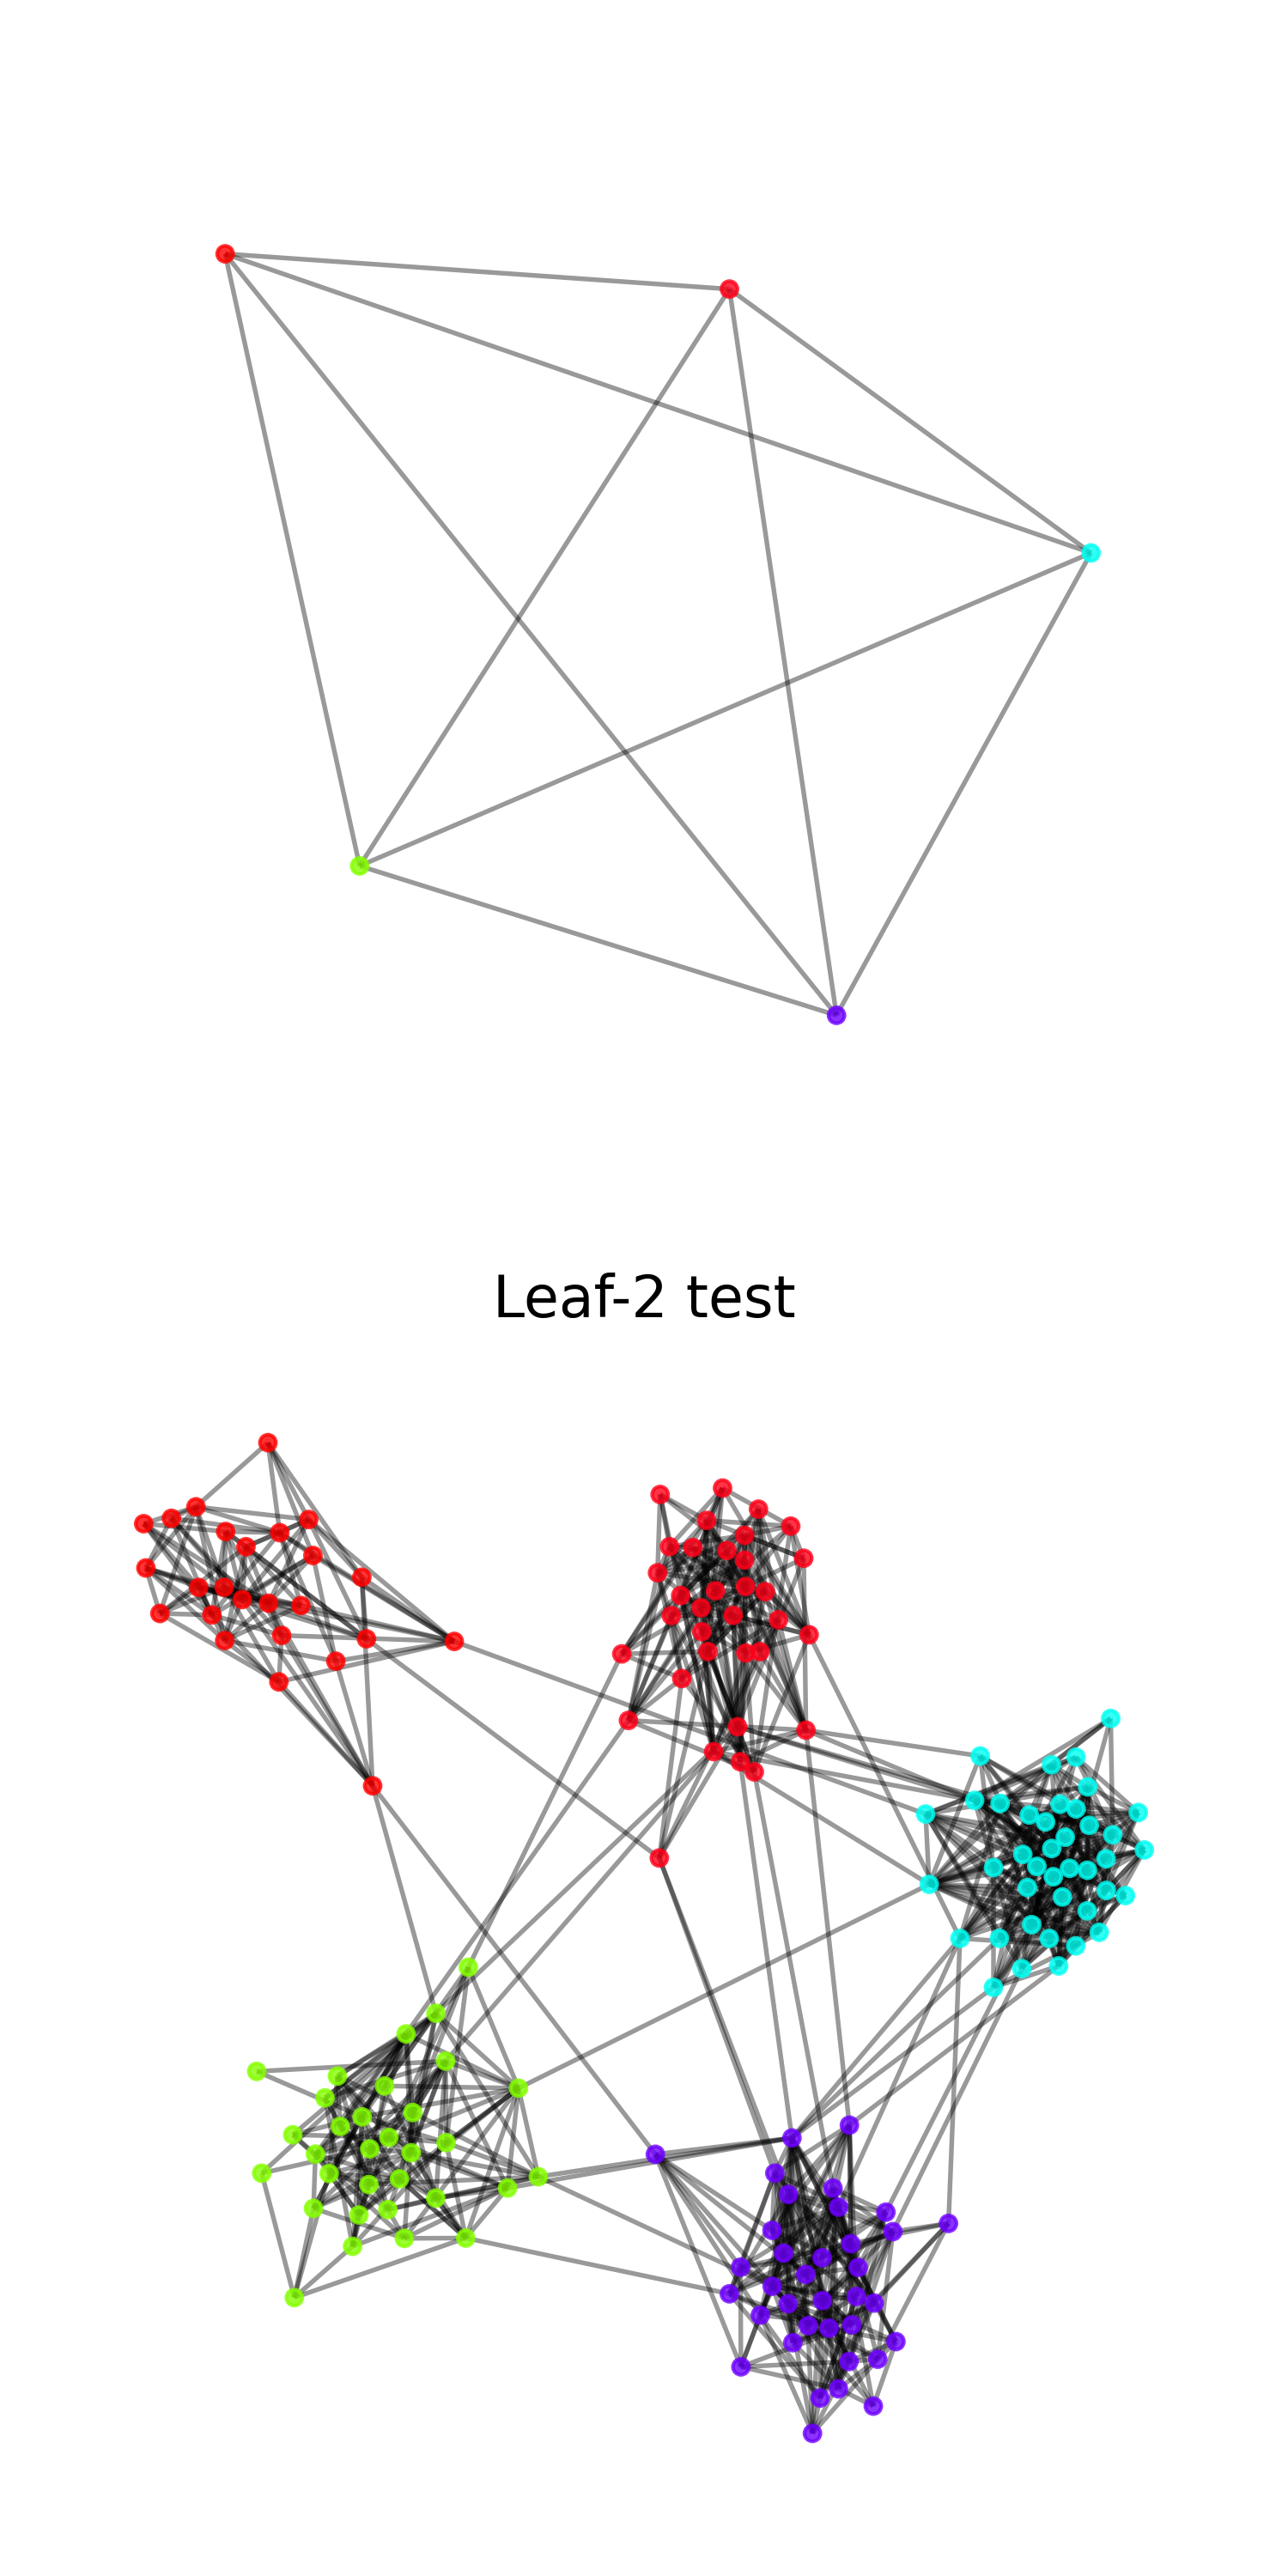
\includegraphics[width=0.15\linewidth]{figures/higendiff/sbm_gen.png}
        \hfill
    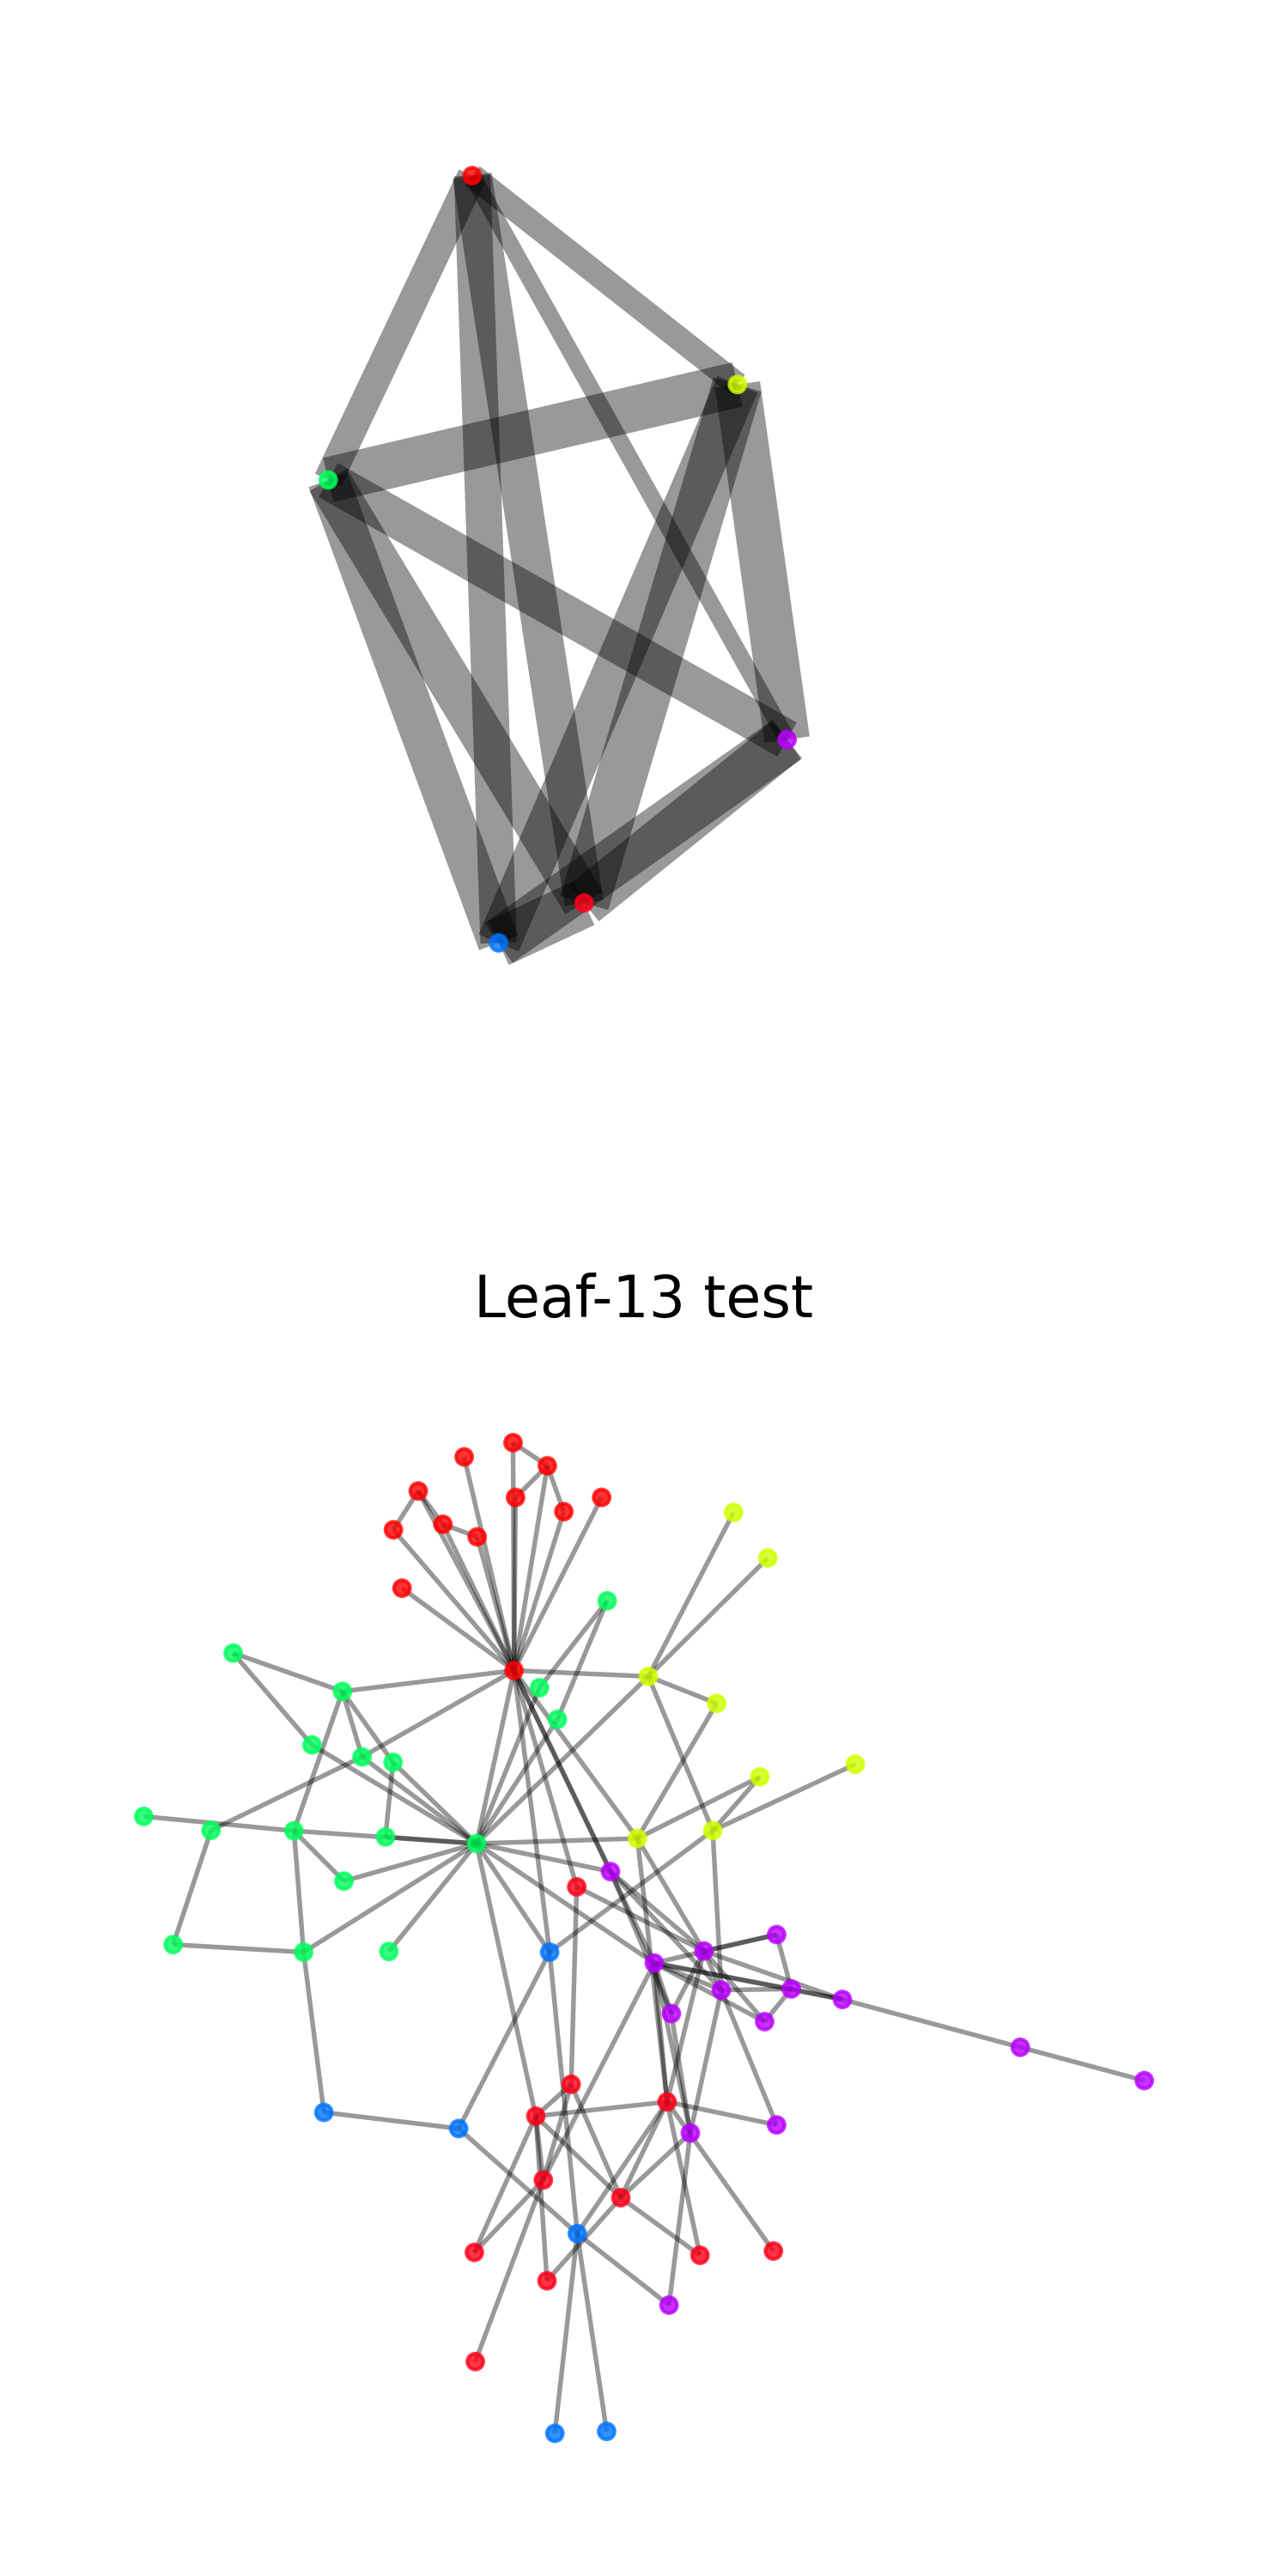
\includegraphics[width=0.15\linewidth]{figures/higendiff/ego2_gen.png}
        \hfill
    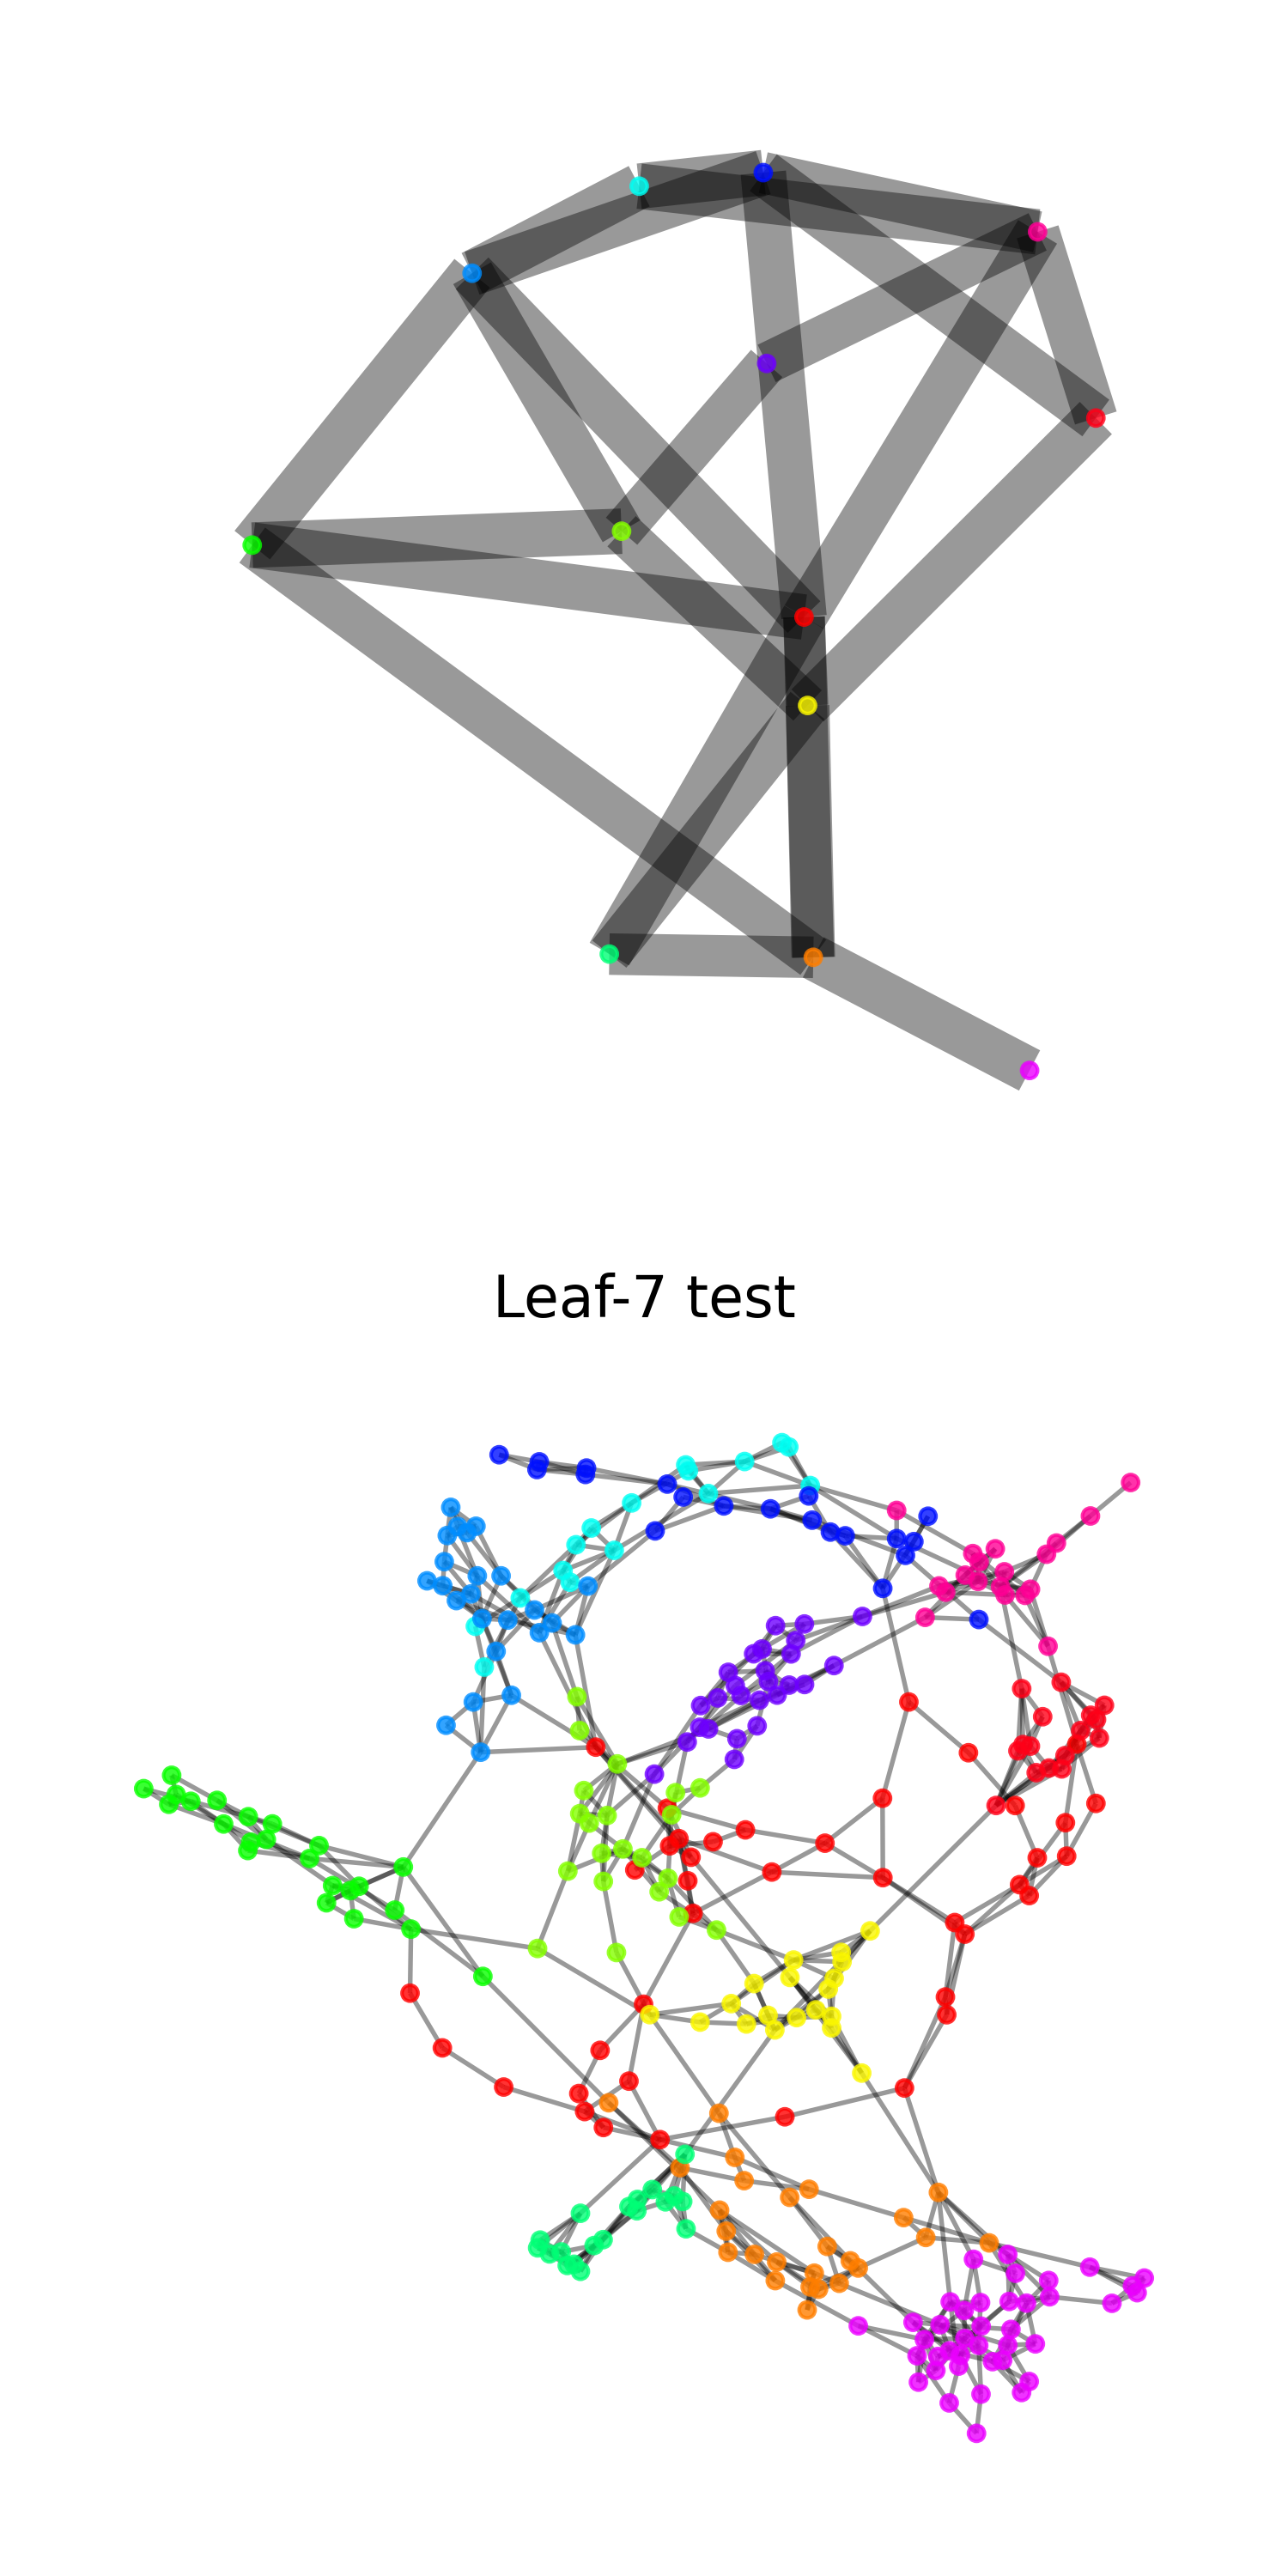
\includegraphics[width=0.15\linewidth]{figures/higendiff/dd2_gen.png}
        \hfill
    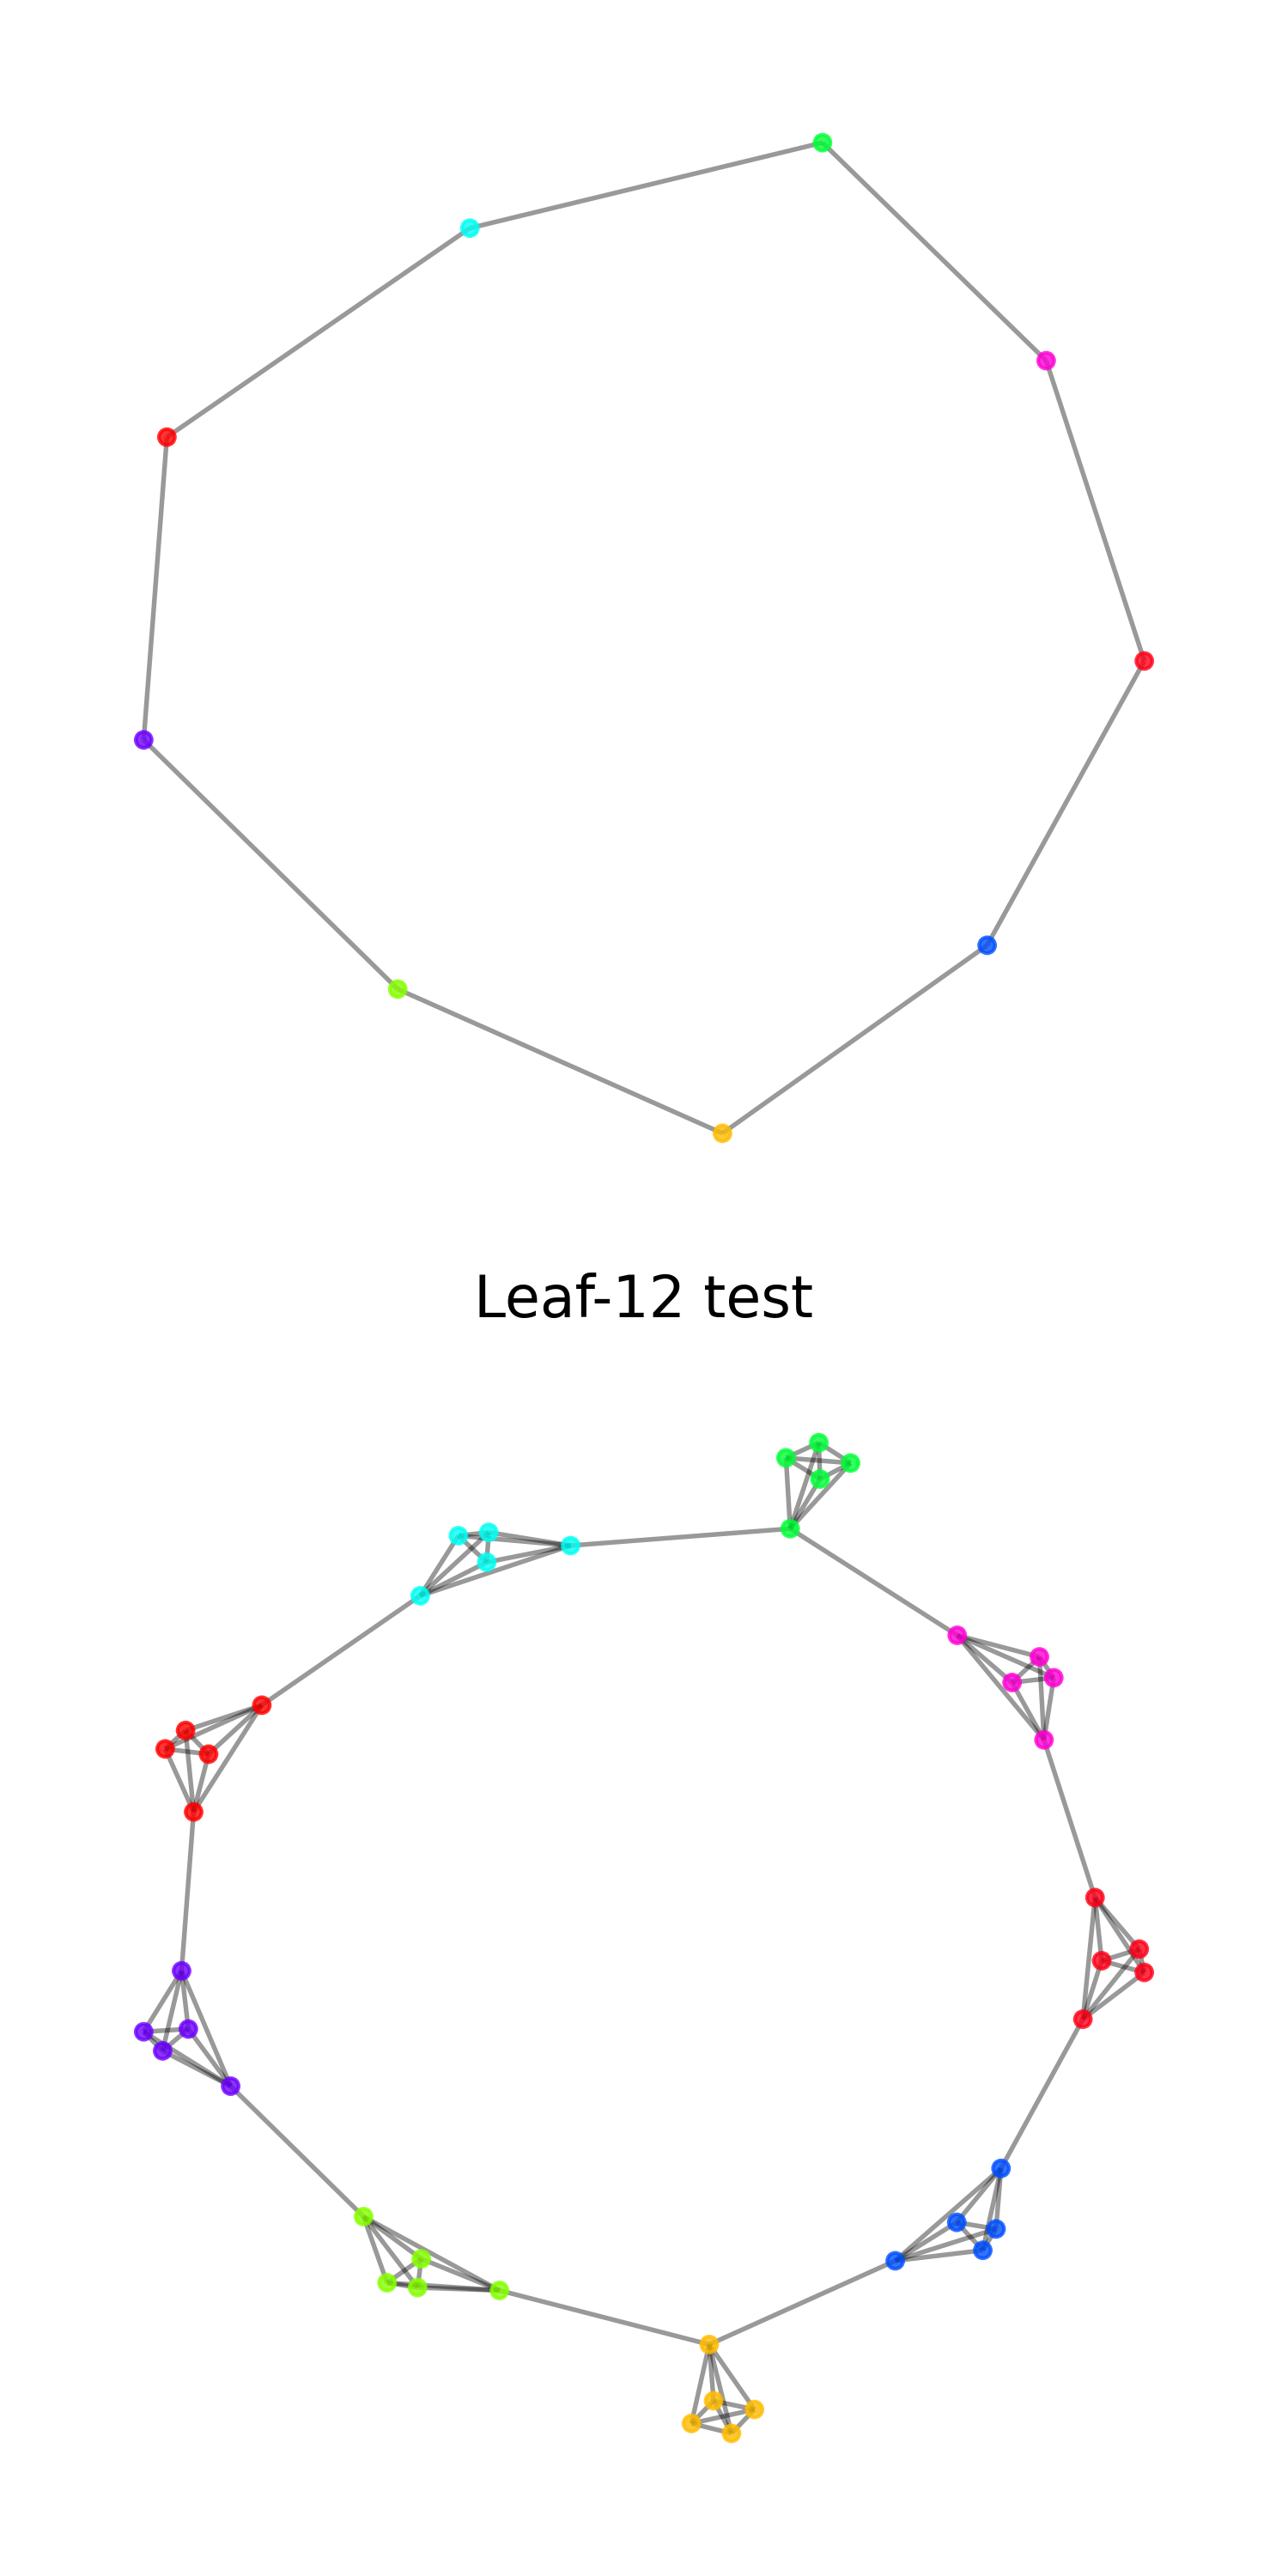
\includegraphics[width=0.15\linewidth]{figures/higendiff/roc_gen.png}
        \hfill
    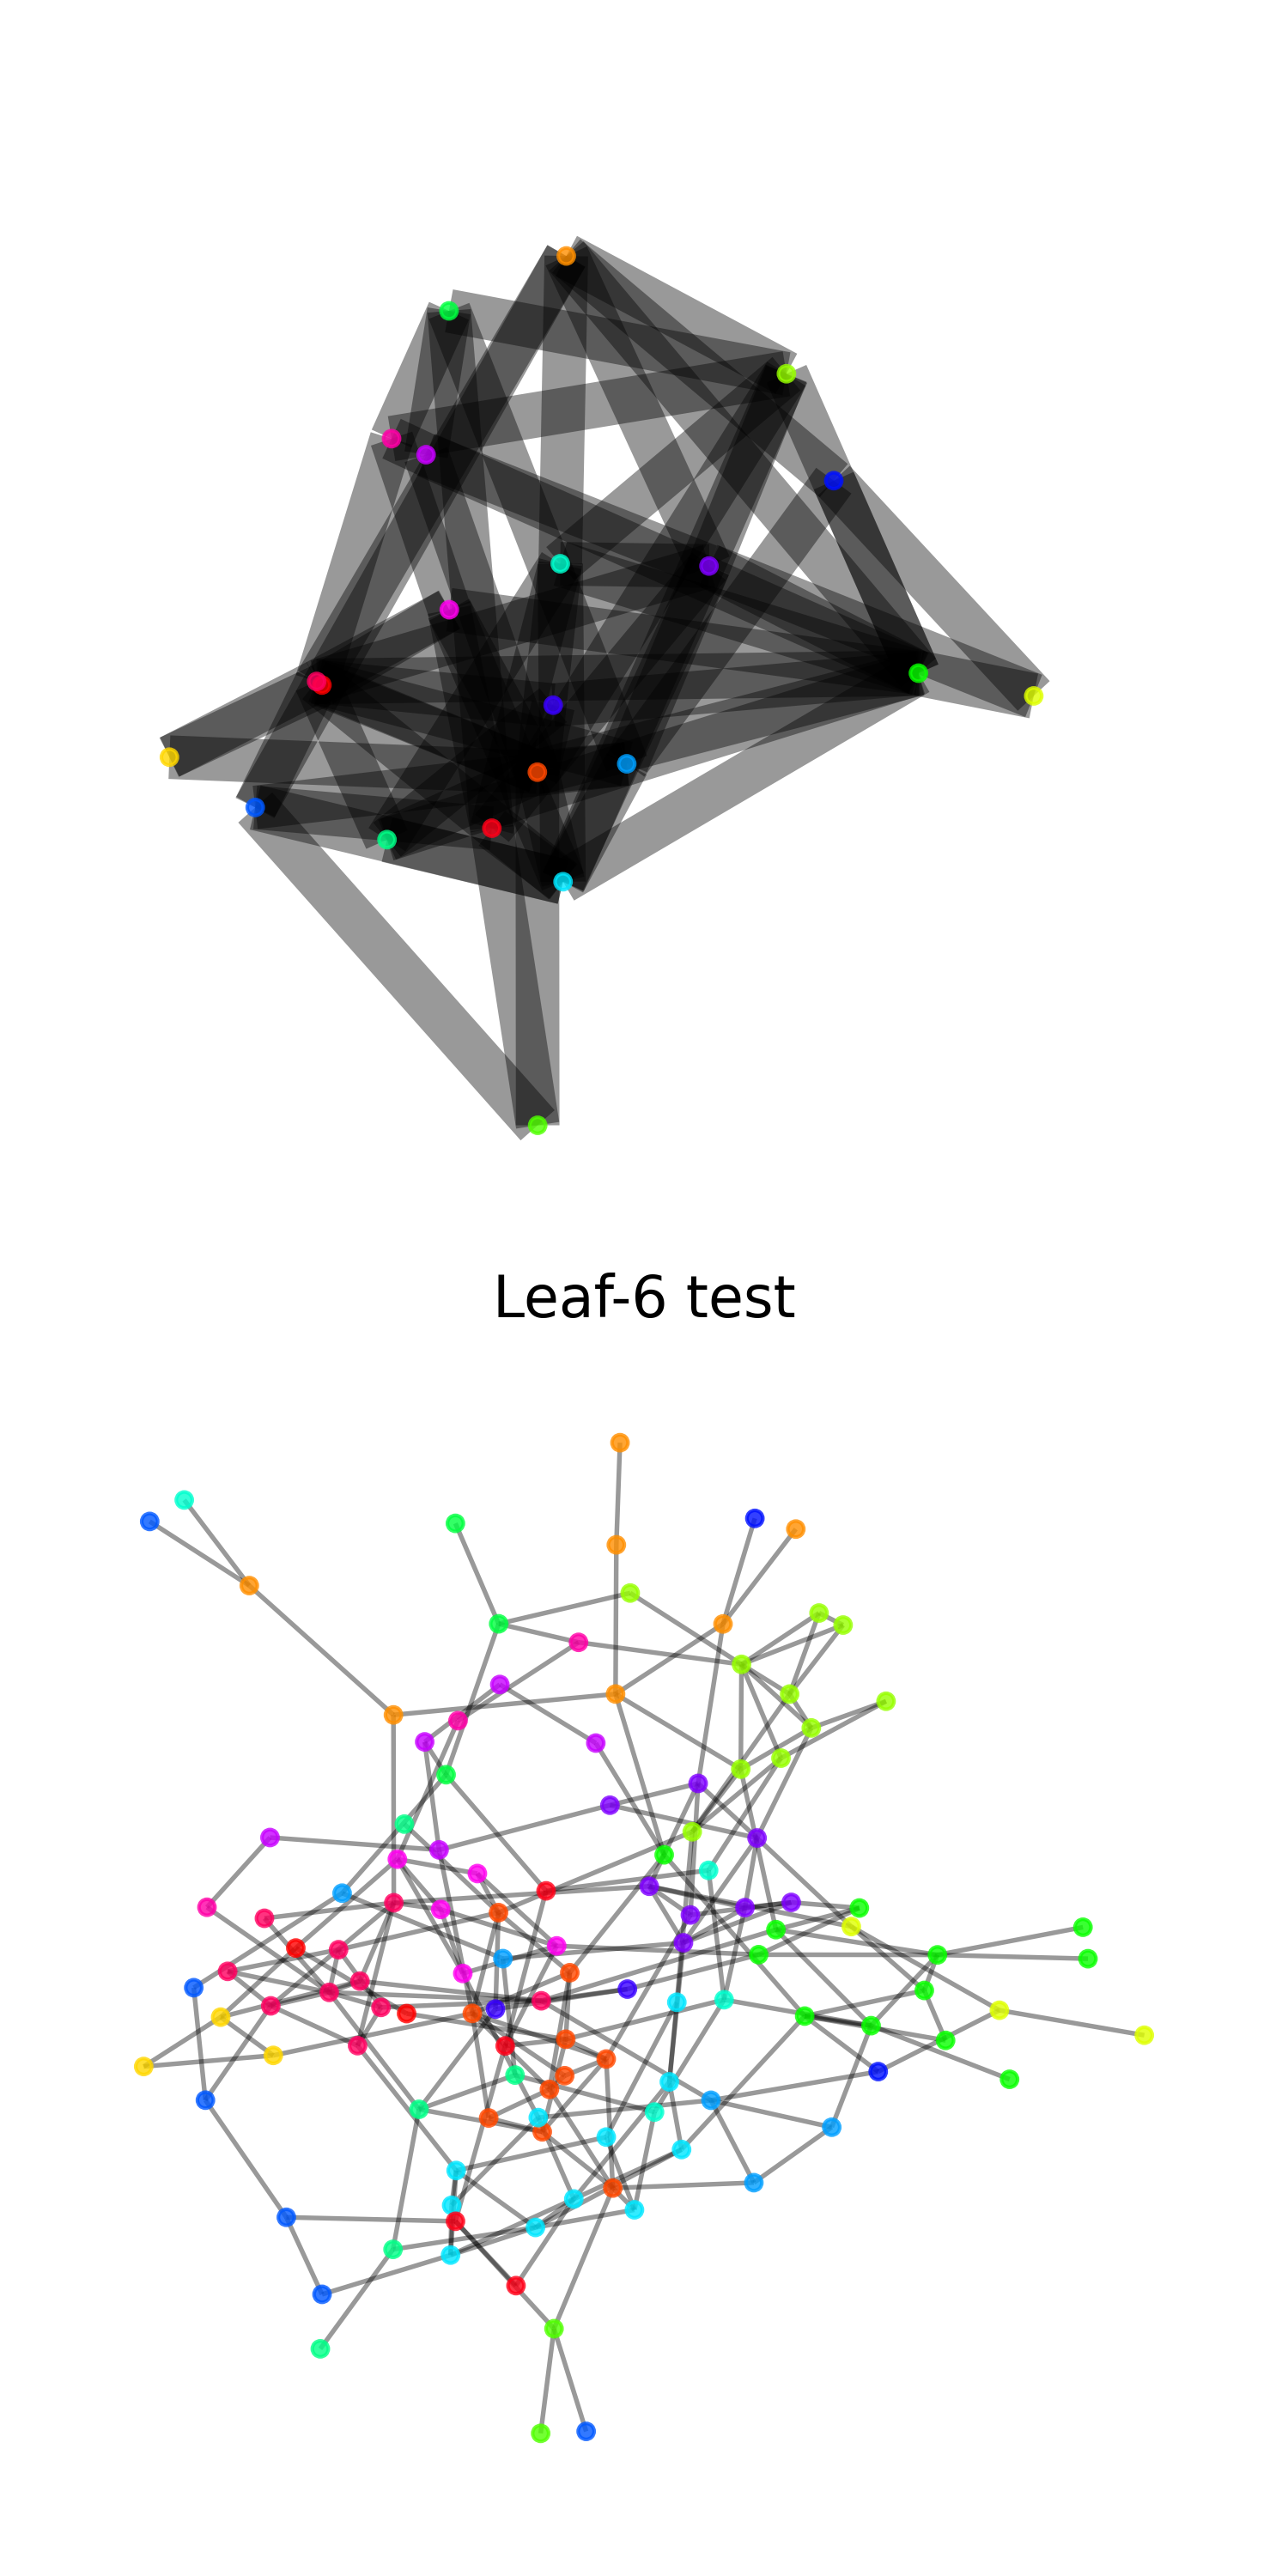
\includegraphics[width=0.15\linewidth]{figures/higendiff/lfr_gen.png}
    \caption{Visual examples of hierarchical graph structures from each dataset. Top vs bottom: real vs sampled graphs. Left to right: different datasets.}
    \label{fig:higendiff_examples}
\end{figure}

\subsection{Summary}

In this section, we introduced Hierarchical Generative Diffusion (HiGenDiff) models, a framework that leverages the inherent hierarchical modularity observed in real-world graph data. Our evaluations demonstrate its promising potential, but work remains in further tuning, detailed evaluation on more datasets, and rising above remaining strong baselines.

HiGenDiff is the mirror image of COINs from the knowledge graph reasoning world into the domain of graph generation. The approach towards success remained the same: both the whole and the parts tell a different, yet equally relevant story, and we must make sure to hear all of the words so as not to lose track of the plot.